Přehled současného stavu je nejprve věnován popisu extrémního prostředí a jeho
vlivu na neuropsychofyziologii (\gls{NPF}) člověka. Dále je na tuto oblast
navázáno popisem kognitivní zátěže (\gls{CL}) v dílčí kapitole kognitivních
neurověd, která tvoří důležitou část problematiky ročníkového projektu a
diplomové práce. Závěr kapitoly je věnován rozboru periferních biosignálů,
jejichž znalost a informační obsah jsou nezbytnými kritérii pro hodnocení
kognitivní zátěže.

\section{Extrémní prostředí}
\label{sec:extreme_environment}
Vzhledem k nejednoznačné definici pojmu \textit{\enquote{extrémní prostředí}} je
potřeba stanovit vhodnou interpretaci v souvislosti s problematikou této práce.
Mezi rané definice přispěli Harrison a Connors~\cite{harrison1984}, kteří
publikovali, že extrémní prostředí se vyznačuje nebezpečnými a nepřívětivými
klimatickými, životními nebo pracovními podmínkami a možnou sociální izolací.
Bell~et~al.~\cite{bell2016} definovali extrémní situace jako okolnosti, za
kterých má nedostatečný výkon, ať už mentální nebo fyzický, vážné následky
(např. časová tíseň, nebo nebezpečí). Všechny tyto koncepty se týkají náročných
fyzických nebo mentálních výkonnostních situací, na které se pojí další již
formulované pojmy jako mimořádné
situace~\cite{stachowski2009benefits,yu2008misery}, psychický a fyzický
nátlak~\cite{gardner2012performance} nebo stres~\cite{Staal2013StressCA}. Další
formulace byly již uvedeny
v~\cite{hannah2009framework,hallgren2018matter,golden2018teams}. V této práci je
na definici extrémního prostředí nahlíženo jako na izolované atypické prostředí,
v němž jsou kladeny značné nároky na plněné úkoly, které s sebou nesou vysokou
míru rizika a katastrofické důsledky při chybném či nedostatečném výkonu.

Současné studie se v rámci tématiky extrémního prostředí často zabývají vlivem
izolovaného a stísněného prostředí (\gls{ICE}, isolated, confined, and extreme)
na člověka~\cite{Pagel2016,golden2018teams} nebo vlivem různorodých
enviromentálních podmínek~\cite{Taylor2016,Winnard2019,Zhang2019}. Do výzkumu v
této oblasti se začalo aktivně přispívat kolem první poloviny 20. století, což
bylo podmíněno vědecko-technologickým pokrokem. Mezi hlavní iniciační milníky
patřil vojenský zájem o dlouhodobé ponory jaderných ponorek, na který navázal
podvodní výzkum~\cite{Maynard2018,Driskell2018}, vznik vesmírných programů
(vesmírný závod) a polární výzkum~\cite{wickman2008,stuster2007bold}. Pro
potřeby této práce je dále detailněji rozebíráno extrémní prostředí z hlediska
vesmírné explorace, konkrétně dlouhodobých vesmírných letů a analogových
vesmírných misí.

\subsection{Vesmírné explorace}
\label{subsection:vesmirne_explorace}
Za hlavní hnací historický faktor, který posouval vědecko-technickou sféru v
rámci výzkumu vesmíru rychle kupředu lze považovat tzv. vesmírný závod, jenž
začal vypuštěním družice Sputnik 1 Sovětským svazem v roce 1957. Rok poté byl
založen Americký Národní úřad pro letectví a vesmír (\gls{NASA}), což vedlo k
prvním vesmírným misím, kterých se později účastnily i posádky. Byl tak vytvořen
nový prostor a vzbuzen výzkumný zájem v oblasti analogových vesmírných misí,
jelikož otázky ohledně průzkumu vesmíru odhalily spoustu vědomostních nedostatků
potřebných pro úspěšný pobyt v kosmu~\cite{Driskell2018}. Nejedná se však ani
tolik o technické překážky, ale o nedostatky znalostí zejména v oboru neurověd a
experimentálního nastavení.

\begin{figure}[!htb]
    \begin{center}
        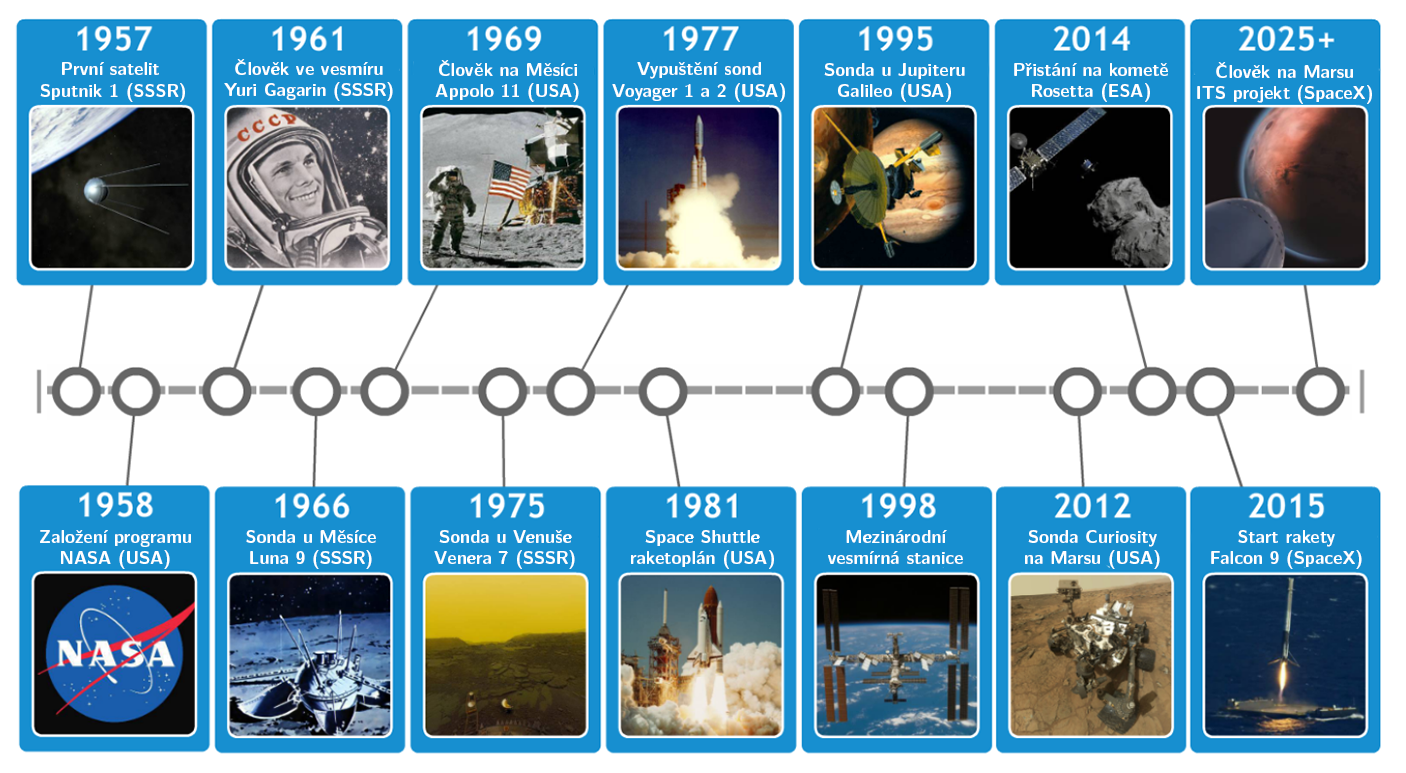
\includegraphics[width=1\linewidth]{figures/space_exploration}
        \caption{Časová osa výzkumu vesmíru od Sputniku po Mars (Přeloženo a
            převzato z~\cite{bartu})}
        \label{fig:space_exploration}
    \end{center}
\end{figure}

Vzhledem k tomu, že budoucnost výzkumu vesmírné explorace sahá za hranice oběžné
dráhy Země~\cite{salotti2014roadmap,viscio2014methodology}, je třeba brát v
úvahu obtíže budoucích misí, které se budou primárně týkat člověka. Dlouhodobé
kosmické lety a mise jsou předmětem mnoha zásadních okolností, jež kladou vysoký
a rizikový neuropsychofyziologický nátlak~\cite{Mogilever2018}. Extrémní
prostředí, komunikační latence a problémy (např. dlouhodobý výpadek komunikace)
nebo fyziologické změny vlivem vesmírných
aspektů~\cite{Buguet2007,Williams2009,Roy2021} mohou během dlouhodobých misí
překračovat lidské psychické i fyzické hranice a vést ke katastrofickým
následkům~\cite{Strangman2014,Mogilever2018}. Toto riziko se uplatňuje i
přestože se v těchto případech skládají posádky z vybraných trénovaných jedinců
(astronautů). Stresory, vnitřní nebo vnější stimuly vznikající při vystavení
lidského organizmu mimořádným podmínkám (extrémnímu prostředí) při dlouhodobých
vesmírných letech, již popsal Morphew~\cite{morphew2001psychological}. Zdravotní
a výkonnostní rizika lze řešit právě výběrem a výcvikem posádky nebo například
návrhem mise a vybavení. Naskytuje se ale také možnost tato rizika predikovat s
využitím diagnostických neinvazivních metod, mezi které patří funkční magnetická
rezonance~(\gls{fMRI}) nebo elektrokardiografie~(\gls{EKG}), spolu s širokými
znalostmi lidského nervového systému. Je tedy třeba realizovat experimenty,
které pomohou lépe chápat, ne-li přímo definovat NPF vztahy při vlivu extrémního
prostředí. Takové experimenty však nemohou probíhat za normálních laboratorních
podmínek, jelikož se nejedná o prostředí, které by odráželo skutečné provozní
podmínky a účinně napodobilo kosmickou misi~\cite{Mogilever2018,Pagel2016}.

Ke studiu neuropsychofyziologických adaptací člověka vystavenému mikrogravitaci
se využívají data zaznamenaná před a po vesmírném letu, kde se také sledují
změny jako distribuce tělesných tekutin, hustota kostí nebo úbytek svalové
hmoty~\cite{Stein2012WeightMA}. Kromě mikrogravitace lze mnoho vědeckých otázek
týkajících se kognitivních neurověd zodpovědět i na Zemi díky vesmírným
analogovým misím, které simulují komplexní interakce vznikající během vesmírných
misí~\cite{Pagel2016,Mogilever2018}.

\subsection{Analogové mise}
\label{subsection:analogove_mise}
Jak již bylo zmíněno, laboratorní experimenty plně nereprezentují reálné
podmínky dlouhodobých kosmických misí, avšak různá analogová prostředí
(analogové mise) přinášejí právě tu možnost sledovat a zkoumat NPF člověka v
jedinečných situacích~\cite{Mogilever2018}. Situace, které napodobují reálné
okolnosti budoucích vesmírných misí -- přistání kosmické lodi, extravehikulární
aktivity (\gls{EVA}), lékařské zákroky aj. -- vystavují jedince pozorovatelným
změnám například v cirkadiánním\footnote{Cirkadiánní rytmus je biologický rytmus
s cyklem trvajícím přibližně jeden den.} rytmu, hladinách stresových hormonů,
imunitních funkcích nebo neurokognitivním změnám~\cite{Pagel2016,Taylor2016}.
Faktory prostředí a jejich vliv na \gls{NPF} jsou detailněji popsány v
následující kapitole.

\begin{figure}[!htb]
    \begin{center}
        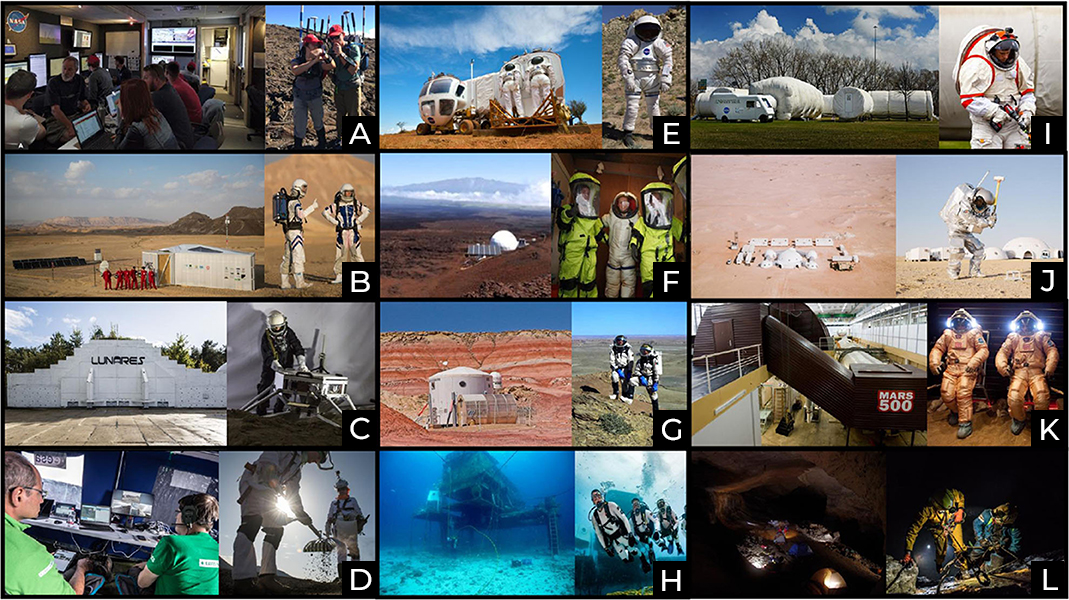
\includegraphics[width=1\linewidth]{figures/analog_missions}
        \caption{Příklady analogových misí. \textbf{(A)} NASA BASALT (USA),
            \textbf{(B)} D-MARS (Izrael), \textbf{(C)} LUNARES (Polsko),
            \textbf{(D)} ESA/PANGEA (Španělsko), \textbf{(E)} NASA/D-RATS (USA),
            \textbf{(F)} HI-SEAS (USA), \textbf{(G)} Mars Desert Research Station
            (USA), \textbf{(H)} NASA/NEEMO (USA), \textbf{(I)} NDU Habitat (USA),
            \textbf{(J)} OeWF/AMADEE-program (Rakousko, Omán), \textbf{(K)} Mars-500
            (Rusko), \textbf{(L)} ESA/CAVES (Španělsko/Itálie). (Upraveno a převzato
            z~\cite{groemer2020})}
        \label{fig:analog_missions}
    \end{center}
\end{figure}

Přehled několika analogových misí, na jejichž vzniku a vývoji se převážně
podílejí: Evropská kosmická agentura (\gls{ESA}), Státní korporace pro kosmické
aktivity (ROSCOMOS), Kanadská kosmická agentura (\gls{CSA}) a \gls{NASA}, lze
vidět na obrázku~\ref{fig:analog_missions}. Každá analogová mise vnikla primárně
pro simulaci a studium určitých vlivů vesmírných podmínek nebo k testování
specifického vybavení. Antarktické mise slouží k testování astrobiologických
hypotéz~\cite{Mogilever2018} a studiu dopadů izolace na člověka během extrémních
podmínek, které jsou dané drsným polárním podnebím a rozsáhlou
tundrou~\cite{Barkaszi2016,lugg1999}. Významnou misí je projekt Mars-500, kde
byla šestičlenná posádka uzavřena 520 dní v napodobenině kosmické lodi pro účely
simulace vesmírného letu na Mars. Během této mise došlo k řadě experimentů,
které se například zabývaly vlivem fyzického cvičení na aktivitu prefrontální
kortexu a kognitivní výkonnost~\cite{schneider2013} nebo změnami nálady a
plazmatických hladin hormonů~\cite{wang2014}. Na základě problematiky této práce
jsou nadále popsány vybrané podvodní analogové mise.

\subsubsection*{Projekt NEEMO}
Operace \gls{NASA} v extrémním prostředí neboli \gls{NEEMO} (NASA Extreme
Environment Mission Operations) jsou analogové vesmírné mise, které probíhají v
Mezinárodní Univerzitní Podmořské Výzkumné Laboratoři na Floridě (Florida
International University's Aquarius Undersea Research Laboratory, \gls{FIU}
\gls{AURL}). Podvodní laboratoř s rozlohou zhruba \SI{43}{\metre\squared},
umístěná \SI{19}{\metre} pod mořskou hladinou přesně nenapodobuje vesmírné
podmínky, ale primárně stresové faktory spojené s bezpečností, komunikací a
technologickou logistikou při dlouhodobých kosmických letech a průzkumu. Zároveň
zde probíhají testy vybavení a trénování výstupu do vesmíru mimo kosmickou
loď~\cite{trembanis2012neemo,koutnik2021neemo}. Poslední mise v podvodní
laboratoři, \gls{NEEMO} 23, proběhla v červnu 2019 a byla primárně zaměřena na
průzkumné výstupy do vesmíru.

\begin{figure}[!htb]
    \centering
    \begin{minipage}[b]{.48\linewidth}
        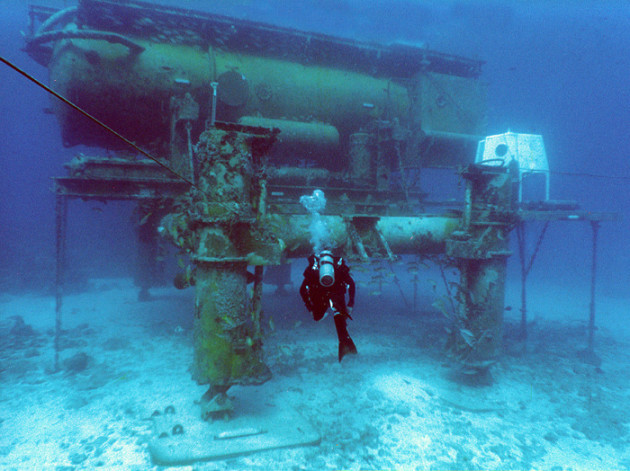
\includegraphics[width=\linewidth]{figures/neemo_habitat}
        \caption{Podvodní habitat AURL~\cite{NASAneemo}}
    \end{minipage}
    \hfill
    \begin{minipage}[b]{.48\linewidth}
        
\includegraphics[width=\linewidth]{figures/hydronaut}
        \caption{Hydronaut H03 DeepLab~\cite{ESAhydronaut}}
    \end{minipage}
\end{figure}

\subsubsection*{Projekt Hydronaut}
Skromnější verze mobilního podvodního habitatu vznikla i v České republice za
účelem výcviku astronautů Evropské kosmické agentury. Projekt byl představen
roku 2010 a jeho primárním cílem bylo umožnit menším posádkám dlouhodobý pobyt
v hyperbarickém \gls{ICE} prostředí a simulaci vesmírných scénářů pro potřeby
výzkumu a vývoje. Podvodní stanice Hydronaut je plně mobilní a lze měnit její
umístění a hloubku zanoření. Současná stanice (H03 DeepLab) je vybavena několika
systémy pro sledování stavu habitatu a posádky. Jedním ze systémů je platforma
Common Tongue, který umožňuje nejen komunikaci s posádkou ale také sledování
fyziologických funkcí. V roce 2020 proběhla desetidenní mise (Mission One),
která včetně účelů kosmického \gls{ICE} výzkumu sloužila jako zátěžový test
habitatu~\cite{hydronaut2014}.


\subsection{Faktory prostředí a změny CNS}
\label{subsection:faktory_prostredi_zmeny_cns}
Vzhledem k tomu, že vesmír je jedinečné prostředí, je studium změn \gls{CNS}
člověka souvisejících s kosmickými misemi obtížné. Předchozí studie ukázaly, že
po letu do vesmíru dochází ke změnám ve vnímání, pohybu, koordinaci a
kognici~\cite{Moore2019}. Mikrogravitace je jedním z hlavních faktorů, které
ovlivňují mozek včetně kosmického záření (radiace), izolace nebo
hyperkapnie~\cite{Roy2021}. Důsledky působení mikrogravitace na mozek popsal
Torre v~\cite{Torre2014}. Souhrn faktorů lze vidět na
Obrázku~\ref{fig:factors_neuro} a jejich počet nasvědčuje, že pozorované
\gls{NPF} změny u astronautů mohou být důsledkem kombinace více stresorů na
jednotlivé oblasti mozku~\cite{Roy2021}.

Nedávné MRI studie poukázaly na změny polohy mozku, objemu tkáně, objemu
mozkových komor, distribuce a dynamiky mozkomíšního moku, mikrostruktury tkáně a
funkční konektivity po letu do
vesmíru~\cite{Ombergen2019,Pechenkova2019,Roberts2017,Demertzi2015,Kramer2020}.
Přehled \gls{MRI} studií provedených na amerických astronautech a ruských
kosmonautech před a po kosmickém letu se zjištěnými poznatky byl vypracován
v~\cite{Roy2021}. Mezi tyto studie jako jeden z prvních přispěl Demertzi et
al.~\cite{Demertzi2015} s objevem snížené konektivity v pravé
insule\footnote{Insula neboli insulární kortex je složitá struktura s rozsáhlou
sítí korových a podkorových oblastí mozku, které slouží smyslovým, emočním a
kognitivním funkcím.}, který se podílí na vestibulárním zpracování a kognitivní
kontrole.

Neurozobrazovací studie na zvířecích modelech a lidech vystavených analogovým
vesmírným letům prokázaly změny mozku související s reálným kosmickým
letem~\cite{Kramer2020,Correia1998}. Analogové vesmírné mise nacházejí tedy
uplatnění při zkoumání vlivů stresorů spojených s vesmírným prostředím na
centrální nervovou soustavu (CNS). Při srovnání změn CNS souvisejících s
kosmickou misí se změnami pozorovanými u pozemských analogů se naskytuje
příležitost do budoucna navrhnout strategie a opatření, které by předcházely
nežádaným NPF účinkům. Během analogových misí se podařilo reprodukovat například
zjištění spojené se změnami mozkové konektivity, objemu šedé hmoty, dynamiky
mozkomíšního moku a objemu mozkových komor~\cite{Roy2021}. Metoda, která věrně
napodobuje podmínky kosmických letů vystavováním subjektů posunu tělních
tekutin, odlehčení axiálního tlaku nebo hypokinezi, se nazývá Head-Down Bed Rest
(\gls{HDBR}). Subjekt je během metody na lůžku hlavou dolu, pod určitým
náklonem. HDBR zároveň vyvolává podobné změny v mozkové konektivitě, včetně
změny konektivity motorických, somatosenzorických a vestibulárních oblastí mozku
jako při vesmírných letech~\cite{Koppelmans2016, Koppelmans2017}.

\begin{figure}[!htb]
    \begin{center}
        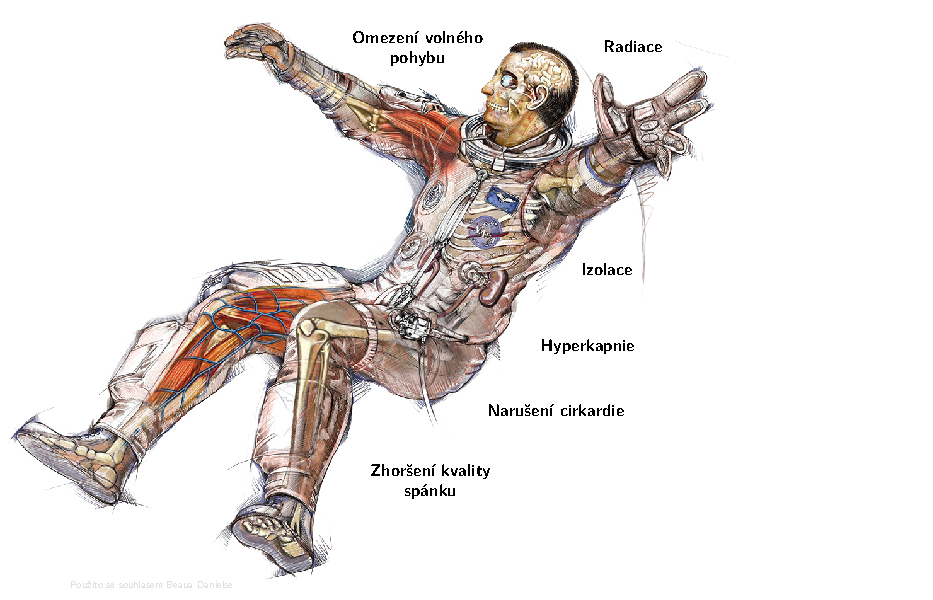
\includegraphics[width=1\linewidth]{figures/space_stressors}
        \caption{Souhrn stresových faktorů vesmírného \gls{ICE} prostředí, které
            mohou ovlivnit mozek během kosmického letu. Radiace* v tomto případě
            odkazuje na radiaci v otevřeném kosmickém prostoru, nikoli na nízké
            oběžné dráze (\gls{LEO}). (Upraveno a převzato
            z~\cite{Roy2021,Hodkinson2017} se souhlasem Beaua Danielse)}
        \label{fig:factors_neuro}
    \end{center}
\end{figure}

Mozek je kromě fyziologických stresorů ovlivněn také dlouhodobým pobytem v
\gls{ICE} prostředí. Po 520denní misi Mars-500 ukázaly snímky participantů
pozměněnou mikrostrukturu šedé hmoty v pravém temporoparietálním
spojení\footnote{Temporoparietální spojení je část mozku, kde se setkávají
spánkový a temenní lalok.} (\gls{TPJ}), což je přisuzováno vlivu izolovaného
prostředí~\cite{Brem2020}. Během dlouhodobých vesmírných misí mohou mít změny
TPJ za následek zhoršení neuropsychofyziologické adaptace člověka na nové ICE
prostředí. Další nežádoucí změny byly prokázány v rámci studií antarktických
expedic, které demonstrovaly snížení objemu šedé hmoty v orbitofrontální kůře,
prefrontální kůře a hipokampu. Vzhledem k povaze antarktického prostředí a
expedic lze usuzovat, že jsou tyto změny podmíněné také vlivem
\gls{ICE}~\cite{Stahn2019}. Možné snížení neurogeneze hipokampu vlivem
extrémního prostředí může mít vliv na paměť a sociální interakci členů
posádky~\cite{Roy2021}. Délka kosmické mise či letu také hraje rozdíl, jelikož
větší míra změn struktury mozku byla pozorována u dlouhodobých vesmírných
misí~\cite{Roberts2017}.

\section{Kognitivní neurovědy}
\label{sec:cognitive_neuroscience}
Lidský mozek je schopen se neustále přizpůsobovat měnícím se okolnostem a
požadavkům prostředí. Astronauti se musí aklimatizovat na zcela nové prostředí
podobně jako malé děti procházejí svými vývojovými fázemi. V podmínkách stavu
beztíže nebo mikrogravitace dochází mimo jiné k ovlivnění mozkových procesů.
Cílem kognitivních neurověd ve vesmíru je pochopit, jak mozek a mysl reagují na
tyto jedinečné okolní podmínky. První výzkumy v oblasti neurověd ve vesmíru byly
provedeny v roce 1962 během ruské mise Vostok-3. Na Zemi je oproti vesmíru možné
díky neurozobrazovacím technikám snadno studovat mozkovou aktivitu a kognitivní
funkce. Pro neurovědce i psychology je velmi důležité pochopit základní
neurokognitivní a neuropsychologické aspekty kosmického letu. Neefektivní
mentální výkon jedince či posádky je známou hrozbou pro vesmírné mise. Pozemský
výzkum zdůrazňuje nutnost porozumět kognitivním procesům, jelikož \gls{CL}
zhoršuje kognitivní a percepční motorické schopnosti. Srovnatelné dopady lze
předpokládat i při vesmírných misích v náročných \gls{ICE} podmínkách a
simulacích (analogové mise)~\cite{Torre2014}. Pro potřeby diplomové práce je
rozsáhlá kapitola kognitivních neurověd vymezena popisu kognitivní zátěže.

\subsection{Terminologie}
\label{subsection:terminologie_CL}
Obor kognitivních neurověd se nachází na pomezí psychologie a neurověd, ale
překrývá se s dalšími obory jako kognitivní a biologická psychologie, fyziologie
nebo neuropsychologie. Tyto obory často studují podobné procesy ale z jiného
pohledu a pomocí jiné metodiky. Synonymem oblasti kognitivních neurověd byl v
této práci zvolen termín neuropsychofyziologie pro usnadnění popisu
fyziologických změn v důsledku kognitivních procesů. Cílem této práce není
rozlišovat mezi jednotlivými obory, ale zaměřit se na vědecké otázky z jejich
průniků, které jsou spojené s vlivem \gls{ICE} prostředí na člověka.

\subsection{Kognitivní zátěž}
\label{subsection:kognitivni_zatez}
Prvotní pojetí kognitivní zátěže (\gls{CL}, Cognitive Load) pochází z oblasti
výuky a vzdělávání, kterou se intenzivně zabýval Sweller et
al.~\cite{Sweller1988,Sweller1998,Sweller2010} kolem přelomu 19. a 20. století.
Sweller~\cite{Sweller1988} jako první formuloval teorii kognitivní zátěže
(\gls{CLT}, Cognitive Load Theory), podle které je \gls{CL} definována jako
zvýšené požadavky na ukládání a zpracování informací v pracovní paměti člověka.
Chen et al.~\cite{Chen2016} definoval kognitivní zátěž jako proměnnou, jež
určuje míru požadavků kladených úkolem na dostupné mentální zdroje pro
zpracování informací. Míra požadavků vychází z vnímané námahy při učení, myšlení
a uvažování jakožto ukazatel zatížení pracovní paměti během plnění úkolu. Tato
míra zároveň popisuje interakce mezi nároky na zpracování úkolu a lidskou
mentální výkonností~\cite{Haapalainen2010}. Ačkoli se definice kognitivní zátěže
v jednotlivých oborech mohou lišit, všechny mají jeden základní prvek: procento
využité kapacity lidské pracovní paměti. Na rozdíl od naší smyslové a dlouhodobé
paměti, které mohou v podstatě neomezeně zpracovávat informace, je tato kapacita
omezená~\cite{Vanneste2021}.

Chen et al.~\cite{Chen2016} publikoval, že vysoká kognitivní zátěž (kognitivní
přetížení) může mít negativní dopad na výkonnost pracovní paměti. Vliv
kognitivní zátěže zároveň ovlivňuje mozkové procesy a kognitivní přetížení
pravděpodobně bezprostředně předchází vyhoření~\cite{Vanneste2021}. Většina
kognitivních funkcí, jako je například selektivní pozornost nebo sebekontrola,
závisí na pracovní paměti. Pracovní paměť zahrnuje aktivní krátkodobé ukládání,
zpracování a manipulaci s informacemi a její efektivní fungování je kriticky
závislé na inhibičních nervových procesech. Nervové středisko pracovní paměti
sestává hlavně z distribuované sítě struktur zahrnující prefrontální kortex jako
důležité ohnisko. 

Variabilita srdeční frekvence (\gls{HRV}) souvisí s aktivitou prefrontální kůry
a je inverzně spojena s aktivitou subkortikálních struktur jako je
amygdala~\cite{Thayer2009}. Vliv kognitivní zátěže se také promítá do
elektrodermální (\gls{EDA}) a respirační (\gls{RSP})
aktivity~\cite{Mogilever2018}. Díky periferním biologickým signálům se tedy
naskytuje jednoduší možnost hodnocení či predikce kognitivních procesů bez
nutnosti použití realizačně a finančně náročnějších neurozobrazovacích metod
nebo elektroencefalografie (\gls{EEG}). Detailněji jsou fyziologické změny
spojené s vlivem \gls{CL} popsány v následující sekci.

\subsection{Fyziologické projevy}
\label{subsec:fyziologicke_projevy_CL}
Z předchozího textu již může být zřejmé, že kognitivní zátěž je velmi úzce
spojená s fyziologickými změnami v lidském organismu. U jedince, kde dojde k
stimulaci CL, může docházet k řadě změn, například v mozkové aktivitě, krevním
tlaku, srdečním rytmu, rychlosti pulzní vlny, dýchaní nebo činnosti potních
žláz~\cite{Vanneste2021,Haapalainen2010,Thayer2009,Gjoreski2017,Cruz2019,Brouwer2015}.
Vybrané fyziologické funkce, do kterých se promítá kognitivní zátěž, jsou
společně s jejich krátkým popisem a neurobiologickým vztahem uvedeny v
Tabulce~\ref{tab:prehled_fyziologicke_projevy_CL_tab1}. Tabulka zároveň
poukazuje na rozdílné vztahy fyziologických parametrů s kognitivní zátěží.

\begin{table}[!htb]
    % \setlength{\tabcolsep}{10pt}
    \renewcommand{\arraystretch}{1.5}
    \centering
    \begin{threeparttable}
        \caption{Přehled vybraných nejčastěji studovaných fyziologických změn a
            stručné teoretické zdůvodnění jejich souvislostí s kognitivní zátěží
            (Upraveno a převzato z~\cite{Vanneste2021})}
        \label{tab:prehled_fyziologicke_projevy_CL_tab1}
        \scriptsize
        \begin{tabular}{p{3cm}p{11cm}}
            \toprule
            Fyziologická funkce & Stručný popis a teoretické zdůvodnění předpokládaného vztahu mezi fyziologickým měřením a kognitivní zátěží
            \\ \midrule
            EEG                 & \textit{Popis}: \gls{EEG} umožňuje měřit mozkovou aktivitu neinvazivně. Provedení spektrální analýzy naměřených rozdílů elektrických potenciálů umožňuje analyzovat výkon různých frekvenčních pásem, která jsou v signálu\newline
            \rule{0pt}{2.5ex}\noindent
            \textit{Hypotéza}: Zvýšení kognitivní zátěže lze měřit zvýšením mozkové aktivity, tj. oscilací v určitém frekvenčním pásmu s větší amplitudou~\cite{Antonenko2010}
            \\
            Eye-tracking        & \textit{Popis}: Měření průměru zornice, latence mrknutí a charakteristik sakád\newline
            \rule{0pt}{2.5ex}\noindent
            \textit{Hypotéza}: Sledování očí bylo v předchozích studiích spojeno s kognitivní zátěží prostřednictvím neurobiologických mechanismů, jako je inervace neuronů autonomního nervového systému radiálními vlákny duhovky~\cite{Wel2018}
            \\
            EDA                 & \textit{Popis}: Elektrodermální aktivita, hodnotí elektrické charakteristiky kůže, aby bylo možné odvodit změny vlivem sympatického nervového systému.\newline
            \rule{0pt}{2.5ex}\noindent
            \textit{Hypotéza}: Kognitivní zátěž má vliv na stres nebo vzrušení a vede ke zvýšení kožní vodivosti~\cite{Setz2010}
            \\
            Teplota pokožky     & \textit{Popis}: Měření teploty vnějšího povrchu lidského těla\newline
            \rule{0pt}{2.5ex}\noindent
            \textit{Hypotéza}: Kognitivní zátěž má vliv na stres nebo vzrušení a vede k vazokonstrikci, což snižuje teplotu kůže~\cite{Herborn2015}
            \\
            EKG                 & \textit{Popis}: Srdeční frekvenci a variabilitu srdeční frekvence lze hodnotit pomocí elektrokardiogramu nebo fotopletysmografie\newline
            \rule{0pt}{2.5ex}\noindent
            \textit{Hypotéza}: Tepová frekvence je měřítkem aktivity sympatického i parasympatického autonomního nervového systému. Stres nebo vzrušení způsobí zvýšení krevního tlaku a snížení variability srdeční frekvence~\cite{Jercic2020,Solhjoo2019}
            \\
            RSP                 & \textit{Popis}: Kognitivní zátěž vede ke zrychlenému dýchání a vyšší minutové ventilaci, přičemž dechová amplituda zůstává stejná\newline
            \rule{0pt}{2.5ex}\noindent
            \textit{Hypotéza}: Při soustředění pozornosti nebo plnění náročného úkolu dochází ke změnám v dýchání~\cite{Grassmann2016}
            \\
            \bottomrule
        \end{tabular}
    \end{threeparttable}
\end{table}

Příkladem rozdílností může být EEG, u kterého je vztah s kognitivní zátěží
přímější než u srdeční nebo elektrodermální aktivity. Hodnocení pomocí tohoto
biosignálů je tedy v některých případech spolehlivější. Pouze v některých,
protože se vychází z předpokladu, že veškeré změny v kognitivních funkcích
člověka se odrážejí v jeho fyziologii~\cite{Vanneste2021}. To znamená, že žádná
měřicí technika nemůže sama o sobě zachytit všechny aspekty kognitivních funkcí
nebo o nich jednoznačně vypovídat. Problematika těchto vztahů je nadále
rozebírána v kapitole~\ref{sec:neurovisceralni_integrace}. Na tuto vícerozměrnou
povahu kognitivní zátěže poukázal Kramer et al.~\cite{Kramer1991}. Dále
definoval kritéria: citlivost, diagnostičnost, rušivost, spolehlivost a obecnost
použití, v rámci kterých bude mít každé fyziologické měření jinou povahu. V
případě kognitivní zátěže a její spolehlivém hodnocení z fyziologických projevů
je proto vhodný multimodální\footnote{Multimodálním přístupem je myšleno využití
více biosignálů.} přístup, který může poskytnout její robustnější
reprezentaci~\cite{Chen2016}.

\subsection{Detekce a hodnocení kognitivní zátěže}
\label{subsec:detekce_CL}
Mezi tří nejčastěji používané způsoby detekce a hodnocení kognitivní zátěže
patří dotazníkové metody subjektivního hodnocení a hodnocení založené na
výkonnosti jedince. Třetím způsobem je právě využití periferních biosignálů.
Subjektivní hodnocení vychází z předpokladu, že hodnocený subjekt je schopen
vnímat své vlastní kognitivní procesy a informovat o případné kognitivní zátěži
nebo o množství vynaloženého mentálního úsilí~\cite{Wang2019,Schnotz2007}. K
subjektivnímu hodnocení se dále využívají specifické dotazníky, mezi které patří
například NASA-TLX. Jedná se o vícerozměrnou stupnici používanou k měření
pracovní zátěže operátorů v rámci úkonů, například během vesmírných analogových
misí~\cite{Sandra2006}. Tyto metody ale nejsou předmětem této práce a jsou
detailně popsány v~\cite{Schnotz2007}.

\begin{figure}[!htb]
    \begin{center}
        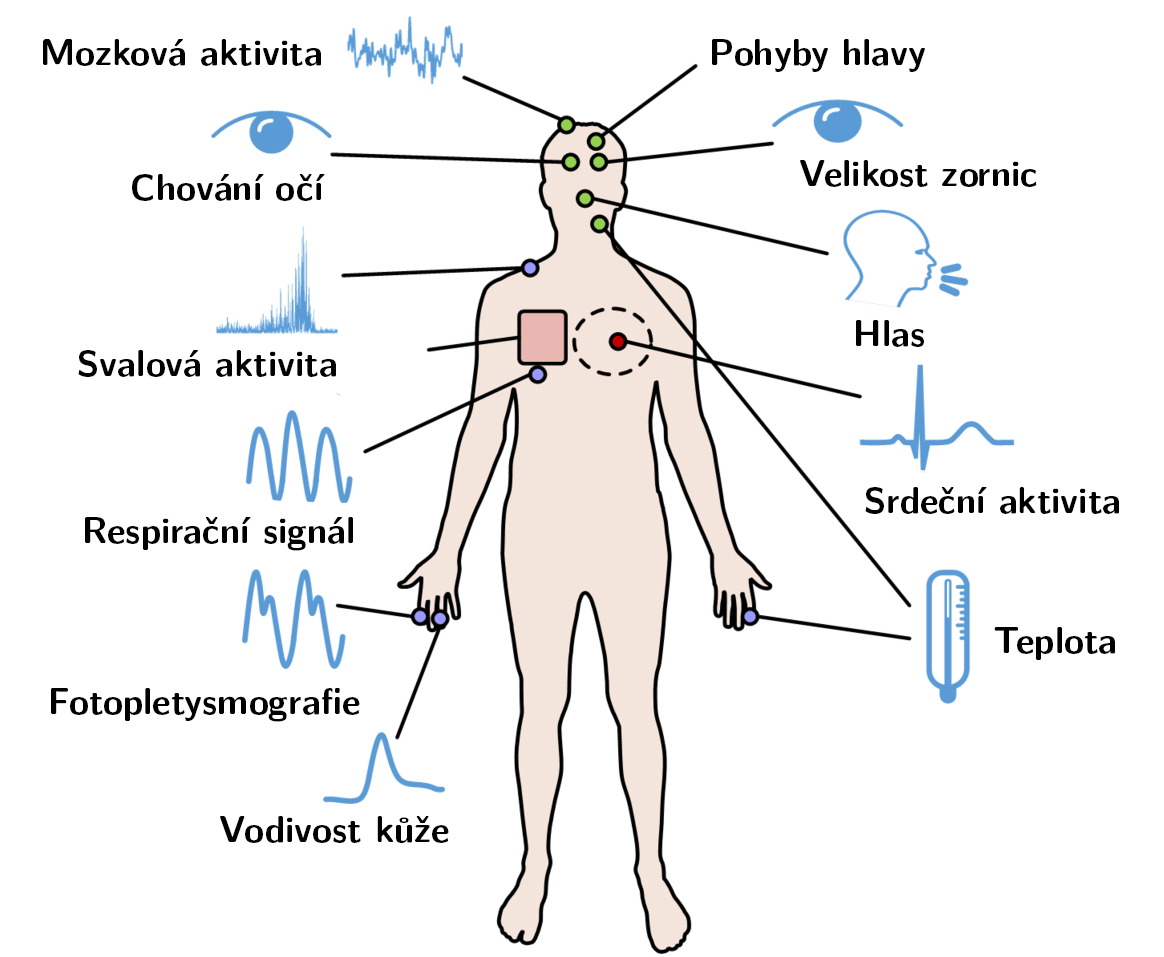
\includegraphics[width=0.85\linewidth]{figures/physiological_measures}
        \caption{Vybrané proměnné související s \gls{CL} (Přeloženo a převzato
            z~\cite{Giannakakis2022})}
        \label{fig:physiological_measures}
    \end{center}
\end{figure}

Na kognitivní zátěž lze nahlížet jako na multidimenzionální konstrukt, který
reprezentuje zátěž vyvinutou na jedince~\cite{Wang2019}. Zároveň se efekt
stimulace kognitivních funkcí u každého jedince projevuje jinak. Nelze tedy
vytvořit žádnou univerzální metodu, která by byla schopná stejně spolehlivě
detekovat kognitivní zátěž u různých subjektů. Proto se v tomto odvětví nabízejí
a velmi často využívají metody strojového učení v rámci kterých nachází výhodné
uplatnění dříve zmíněný multimodální přístup. Biologická data využívaná pro
účely detekce \gls{CL} lze vidět na Obr.~\ref{fig:physiological_measures}.

Vzhledem k tomu, že je strojové učení širokou oblastí, byla tomuto tématu
věnována samostatná sekce~\ref{sec:machine_learning}. Od roku 2010 je hojně
využívána metoda učení s učitelem (viz~\ref{subsubsec:supervised_learning}) pro
účely klasifikace různých patologických stavů a symptomů~\cite{Ishaque2021}.
Nejčastěji využívaným biosignálem je srdeční aktivita, konkrétně variabilita
srdeční frekvence, které se mnohdy používá v kombinaci s elektrodermální
aktivitou~\cite{Wang2019}. Použité příznaky pro klasifikaci (anglicky features)
však hrají důležitou roli při rozlišování základní funkce spojené s jakýmkoli
fyziologickým signálem. Z variability srdeční frekvence je v současnosti možné
vypočítat desítky parametrů, resp. příznaků, se kterými je v těchto úlohách
nutné zacházet velmi opatrně. Jednotlivé \gls{HRV} parametry společně s jejich
pravděpodobným významem byly již popsány
v~\cite{Haapalainen2010,Rohila2020,Pham2021,Bouny2021}. Blíže je problematika
\gls{HRV} parametrů popsána v samotné podkapitole~\ref{subsec:hrv_indices}.

Dříve mezi často používané metody pro účely klasifikace patřili hlavně
rozhodovací stromy (\gls{DT}), lineární diskriminační analýza (\gls{LDA}) nebo
metoda podpůrných vektorů (\gls{SVM})~\cite{Ishaque2021}. Od roku 2018 se ve
výzkumu HRV však stále častěji používá hluboké učení, jehož cílem je zlepšit
automatickou klasifikaci v reálném čase. Tyto techniky poskytují efektivnější
způsob extrakce relevantních informací a zvyšují přesnost klasifikace a současně
snižují počet příznaků potřebných pro klasifikaci v reálném
čase~\cite{Hwang2018,He2019}. O rok později se stalo novým trendem používání
technik učení bez učitele pro klasifikaci psychického stresu s využitím
technologie autoenkodéru~\cite{Oskooei2019}. Dále se mimo jiné začaly hojně
používat samoorganizující mapy (\gls{SOM}), které dokáží efektivně redukovat
dimenzionalitu dat a zároveň indikovat nejcennější\footnote{Implikuje, jak moc
přispívá každý příznak k predikci modelu.} příznaky pro klasifikaci kognitivní
zátěže s vysokou přesností~\cite{Cho2017}. V rámci předzpracování biosignálů pro
potřeby zmíněných technik však neexistuje žádná sjednaná metodika. Stejně tak
ani pro výběr příznaků nebo z jaké metodiky pro detekci vůbec CL ideálně
vycházet. Proto se stále zkouší variace různých algoritmů se snahou o zlepšení
přesnosti klasifikace.

% \begin{table}[h]
%     \centering
%     \caption{Veřejně dostupné datasety sledující kognitivní zátěž (Upraveno a
%         převzato z~\cite{Gjoreski2020})}
%     \label{tab:cl_datasets}
%     \scriptsize
%     \begin{tabular}{lcp{9cm}}
%         \toprule
%         \textbf{Dataset}      & \textbf{Probandi} & \textbf{Biosignály}                                                          \\ \midrule
%         Ascertain             & 58                & ECG, EDA, EEG, aktivační jednotky obličeje                                   \\
%         Amigos                & 40                & EEG, ECG, GSR, video obličeje                                                \\
%         DEAP                  & 32                & ECG, EDA, EEG, EMG, EOG, RSP, TEMP, video obličeje                           \\
%         DECAF-hudba           & 30                & ECG, EMG, EOG, MEG, near-infrared video obličeje                             \\
%         DECAF-video           & 30                & ECG, EMG, EOG, MEG, near-infrared video obličeje                             \\
%         Mahnob                & 30                & ECG, EDA EEG, RSP, TEMP, video, sledování očí, zvuk                          \\
%         Emotions              & 1                 & ECG, EDA, EMG, RSP                                                           \\
%         Laughter              & 34                & ACC, EDA, PPG, TEMP                                                          \\ \midrule
%         Pracovní zátěž řidiče & 10                & GSR, HR, TEMP                                                                \\
%         Řidičský stres        & 24                & ECG, EDA, EMG, RESP                                                          \\
%         Rozptýlení řidiče     & 64                & GSR, HR, TEMP ECG, EDA, EMG, RSP EDA,HR, RSP, výrazy obličeje, sledování očí \\ \midrule
%         \textbf{CLAS}         & 59                & ACC, ECG, PPG, EDA                                                           \\
%         Stress-math           & 21                & ACC, EDA, HR, TEMP, BVP ACC, EDA, HR, TEMP, BVP                              \\
%         Non-EEG               & 20                & ACC, EDA, HR, TEMP, BVP ACC, EDA, HR, TEMP, SpO2                             \\
%         \textbf{WESAD}        & 15                & ACC, EDA, TEMP, BVP, EMG, RSP                                                \\ \midrule
%         CogLoad               & 23                & ACC, EDA, TEMP, RR                                                           \\
%         Snake                 & 23                & ACC, EDA, TEMP, RR                                                           \\ \bottomrule
%     \end{tabular}
% \end{table}

\section{Neuroviscerální integrace}
\label{sec:neurovisceralni_integrace}
Z minulých kapitol vyplývá, že se veškeré kognitivní funkce člověka promítají
zároveň do těch fyziologických. Většina studií, které se věnují detekci a
hodnocení kognitivní zátěže však tento širší kontext nebere v úvahu. Díky tomu
je nedostatek systematického porovnávání indexů HRV (viz následující
kapitola~\ref{sec:hrv}), což činí interpretaci a vyhodnocování výsledků
zdlouhavým a sporným. Problémem je také samozřejmě dříve zmíněný nedostatek dat.
Tato kapitola slouží k zasazení úlohy této práce do širšího obrazu a zároveň pro
zdůraznění důležitosti problematiky samotné. 

V současné době existuje mnoho studií, které vypovídají o tom, že parasympatický
neboli vagový tonus, souvisí s psychologickými a behaviorálními proměnnými i
zdravotním stavem. Studie například odhalily velký počet konzistentních
zjištění, která ukazují, že jedinci s vyšší variabilitou srdeční frekvence mají
větší schopnosti v oblasti regulace emocí~\cite{Appelhans_Luecken_2006,
Butler_Wilhelm_Gross_2006,Ingjaldsson_Laberg_Thayer_2003,Lane_2008,
Melzig_Weike_Hamm_Thayer_2009, Thayer_Brosschot_2005} a dosahují lepších
výsledků v kognitivních úkolech zahrnujících pozornost, pracovní paměť a
inhibiční kontrolu~\cite{Thayer2009,Hansen_Johnsen_Thayer_2003,
Johnsen_Thayer_Laberg_Wormnes_Raadal_Skaret_Kvale_Berg_2003,
Saus_Johnsen_Eid_Riisem_Andersen_Thayer_2006}. Pokud bychom kategorizovali HRV
pouze na dvě úrovně, vyšší a nižší, tak lze s postupem let pozorovat množství
poznatků z hlediska prognostického významu:
\begin{itemize}
    \item \textbf{vyšší HRV} --- \emph{lepší regulace glukózy, lepší funkce osy
              hypotalamus-nadledviny-hypofýza (HPA), snížení zánětu a snížení rizika
              mrtvice, kardiovaskulárních onemocnění a úmrtnosti ze všech
              příčin}~\cite{Brosschot_Thayer_2007,Liao_Carnethon_Evans_Cascio_Heiss_2002,Thayer_Fischer_2009,Thayer_Lane_2007}
    \item \textbf{nižší HRV} --- \emph{afektivní poruchy, deprese a úzkost,
              špatná kardiovaskulární kondice, vyšší riziko infarktu, zvýšená kognitivní
              zátěž}~\cite{Gorman_Sloan_2000,Kemp_Quintana_2013,Kemp_Quintana_Felmingham_Matthews_Jelinek_2012}
\end{itemize}

\begin{figure}[!htb]
    \begin{center}
        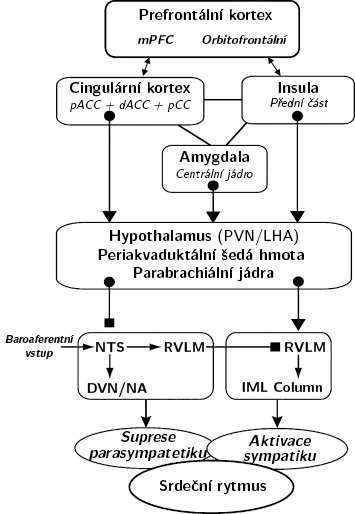
\includegraphics[width=0.9\linewidth]{figures/neurovisceral1}
        \caption{\textbf{(A)} Složené schéma znázorňující dráhy, kterými může
        prefrontální kůra ovlivňovat řízení srdeční frekvence; \textbf{(B)}
        Jádrové oblasti \gls{CAN}, jak je odhalila konjunkční
        analýza\protect\footnotemark\ autonomních modulačních oblastí ve třech
        kategoriích úkolů (barevně označeny). L, levá strana; P, pravá strana
        (Upraveno a převzato z~\cite{gianaros2008,Beissner2013})}
        \label{fig:neurovisceral_diagram}
    \end{center}
\end{figure}

\footnotetext[\thefootnote]{Společné testování více účinků u jednoho subjektu
využitím \gls{fMRI}.}

Objasnění pozorovaných vztahů mezi \gls{HRV} a psychologickými/behaviorálními
proměnnými může v rámci mentálního a fyziologického stavu jedince zlepšit
porozumění a praktickou využitelnost nejen v medicíně. Model
\enquote{\emph{neuroviscerální integrace}} (\gls{NVI}), který v roce 2000
navrhli Thayer a Lane~\cite{Thayer_Lane_2000}, je pokusem o integraci poznatků o
mentálních stavech, autonomních funkcích a zdravotních výsledcích do jednotného
rámce, jehož středobodem je \enquote{\emph{centrální autonomní síť}} (\gls{CAN})
v mozku. \gls{CAN} je síť vzájemně propojených oblastí mozkových
struktur~\cite{Thayer_Lane_2009}. Hlavní části této sítě ukázali pomocí
experimentu Beissner et al.~\cite{Beissner2013} (viz
Obr.~\ref{fig:neurovisceral_diagram}B).

Na diagramu~\ref{fig:neurovisceral_diagram}A lze vidět prefrontální, cingulární a
insulární kůru, jež tvoří propojenou síť s obousměrnou komunikací s amygdalou.
Amygdala je pod tonickou inhibiční kontrolou prostřednictvím prefrontálních
vagových drah k interkalárním buňkám v amygdale. Aktivace centrálního jádra
amygdaly (\gls{CeA}) inhibuje jádro solitárního traktu (\gls{NTS}: plný
čtverec), které následně inhibuje inhibiční vstupy kaudálního ventrolaterálního
medulárního jádra (\gls{CVLM}) do rostrálního ventrolaterálního medulárního
jádra (\gls{RVLM}) sympatoexcitačních neuronů (plný čtverec) a současně inhibuje
vagové motorické neurony v nucleus ambiguus (\gls{NA}) a dorzálním vagovém
motorickém jádru (\gls{DVN}). Kromě toho může CeA přímo aktivovat
sympatoexcitační neurony v RVLM~\cite{gianaros2008}.

\begin{figure}[!htb]
    \begin{center}
        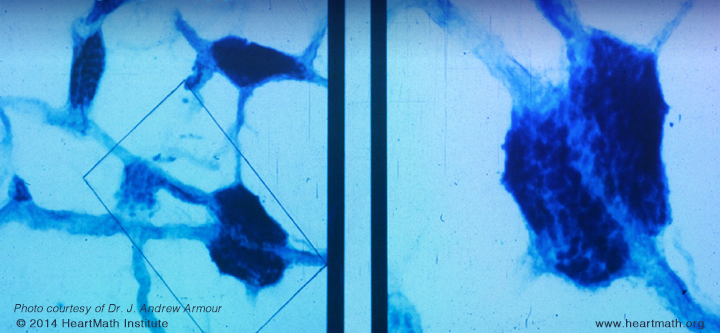
\includegraphics[width=1\linewidth]{figures/cardiac_ganglia}
        \caption{Mikroskopický obraz propojených vnitřních srdečních ganglií v
            lidském srdci. Tenké, světle modré struktury jsou vícenásobné axony,
            které ganglie propojují (Převzato z~\cite{Shaffer2014} se
            souhlasem HeartMath Institutu)}
        \label{fig:cardiac_ganglia}
    \end{center}
\end{figure}

Centrální autonomní síť, tvořena pregangliovými sympatickými a parasympatickými
neurony, inervuje srdce prostřednictvím hvězdicových ganglií a n. vagus. Vlivy
těchto drah na sinoatriální uzel (\gls{SA}) jsou hlavním faktorem určujícím
\gls{HRV}. Vzhledem k rozsáhlým aferentním informacím této autonomní sítě se
promítá úroveň integrace mezi periferním a centrálním nervovým systémem do
\gls{HRV} a poskytuje kontextově specifickou regulaci srdce. Změny autonomních
funkcí, zejména v kognitivních a afektivních souvislostech, odrážejí především
vagový vliv, protože časové měřítko změn tonu sympatiku je relativně pomalejší
než u tonu parasympatiku~\cite{Thayer_Lane_2009,Thayer2009}.

Obrázek~\ref{fig:neurovisceral_diagram}A znázorňuje dráhy, které umožňují
prefrontální kůře regulovat srdeční frekvenci a její variabilitu. \gls{ANS} má
jak tonickou excitační, tak inhibiční kontrolu nad \gls{HR}, kterou může
modulovat frontální kůra prostřednictvím \gls{CeA}. To umožňuje přesnou regulaci
variability srdečního rytmu, která na srdeční úrovní probíhá pomocí
intrakardiálních neuronů (viz Obrázek~\ref{fig:cardiac_ganglia}). Prefrontální
kůra rovněž vykonává tonickou inhibiční kontrolu nad těmito obvody, jak dokládá
inverzní korelace mezi aktivitou ventromediálního prefrontální a orbitofrontální
kortexu a úrovní kožní vodivosti během výchozího stavu mozku\footnote{Základní
stav fyziologického mozku dospělého člověka z hlediska frakce extrakce kyslíku z
mozku neboli OEF~\cite{Raichle2001}.}. To podporuje současný \gls{NVI} model a je
v souladu s pozorováním, kde tyto oblasti jsou deaktivovány během kognitivních
úkolů při současném zvýšení hladiny kožní
vodivosti~\cite{Nagai2004,Raichle2001,Thayer_Lane_2009}.

Souhrnně lze říci, že \gls{NVI} model integruje podstatu periferních
fyziologických změn vlivem specifických mozkových struktur do jednotného
frameworku, který se tyto adaptivní pochody snaží vysvětlit. Podle Thayera a
Lanea~\cite{Thayer_Lane_2000} je tento framework spojen s psychologickými a
fyziologickými procesy prostřednictvím kortiko-subkortikálního neuronálního
okruhu, který lze indexovat pomocí \gls{HRV}. Prefrontální kůra může inhibovat
podkorové struktury, což umožňuje organismu účinně reagovat na požadavky
prostředí~\cite{Thayer_Lane_2009}. Model \gls{NVI} představuje a popisuje
víceúrovňovou funkční strukturu vagové kontroly, jejíž kompletní rozbor ale
přesahuje rozsah této práce. Jednotlivé úrovně dokládají důkazy o souvislosti
mezi \gls{HRV} a fyziologickou, afektivní a kognitivní regulací. Zbytek kapitoly
je proto věnován pouze souhrnu kognitivní regulace. Důkladně byl \gls{NVI} model
rozebrán v literatuře~\cite{Smith_Thayer_Khalsa_Lane_2017,Thayer2009,Thayer_Lane_2009}.

\subsection{Kognitivní regulace}
Schopnost regulovat pozornost a potlačovat nežádoucí reakce (negativní afektivní
stavy) je nezbytná pro přizpůsobení se například právě \gls{ICE} prostředí.
Prefrontální korová aktivita je důležitá pro úkoly vyžadující pracovní paměť,
trvalou pozornost, inhibici chování a mentální
flexibilitu~\cite{Thayer_Lane_2009}. Předchozí studie prokázaly, že jedinci s
vyšší klidovou \gls{HRV} dosahovali lepších výsledků při řešení úkolů (n-back
test, Stroopův test) vyžadujících exekutivní funkce než jedinci s nižší klidovou
\gls{HRV}~\cite{Hansen_Johnsen_Thayer_2003,
Johnsen_Thayer_Laberg_Wormnes_Raadal_Skaret_Kvale_Berg_2003}. Stres může také
zhoršovat kognitivní funkce, přičemž jedinci s nižší klidovou variabilitou
vykazovali horší výkonnost při řešení určitých úkolů, kde byli vystaveni
ohrožení a také větší reakci kortizolu na mírné kognitivní výzvy, které
přetrvávaly i v období zotavení, ve srovnání s jedinci s vysokou klidovou
\gls{HRV}~\cite{Thayer_Lane_2009}.

Saus et al.~\cite{Saus_Johnsen_Eid_Riisem_Andersen_Thayer_2006} ukázali na
realističtějších scénářích zahrnující příslušníky policie, kteří plnili úkoly ve
virtuální realitě, že jedinci s vyšší klidovou \gls{HRV} vykazovali větší
situační povědomí a lepší výkon v plnění úkolu. Kromě toho byl tento krátký
tréninkový program spojen s méně významným snížením \gls{HRV} během plnění
úkolu, což naznačuje snížení mentální zátěže. Tyto výsledky naznačují, že
jedinci s vyšší klidovou \gls{HRV} jsou lépe vybaveni pro plnění úkolů, které
zahrnují exekutivní a inhibiční funkce, a to jak v laboratorním, tak v reálném
prostředí. Navíc naznačují, že trénink může ovlivnit variabilitu srdečního rytmu
a kognitivní výkon.

\section{Variabilita srdeční frekvence}
\label{sec:hrv}
Variabilita srdeční frekvence (\gls{HRV}) vypovídá o časové variabilitě mezi
jednotlivými srdečními stahy a umožňuje nahlédnout do regulace různých tělesných
funkcí autonomním nervovým systémem. Následující kapitola se zabývá způsoby
jakými je možné takové nahlédnutí realizovat a zároveň poukazuje na současné
nedostatky této problematiky, které je třeba brát v potaz. Nejdříve je ale na
místě uvést obecné objasnění vzniku a souvislosti variability srdeční frekvence
s funkcionalitou srdce. Regulační pochody autonomního nervového systému spojené
s \gls{HRV} byly popsány v minulé kapitole (zjednodušeně viz
Obr.~\ref{fig:hrv_diagram}D).

\begin{figure}[h]
    \begin{center}
        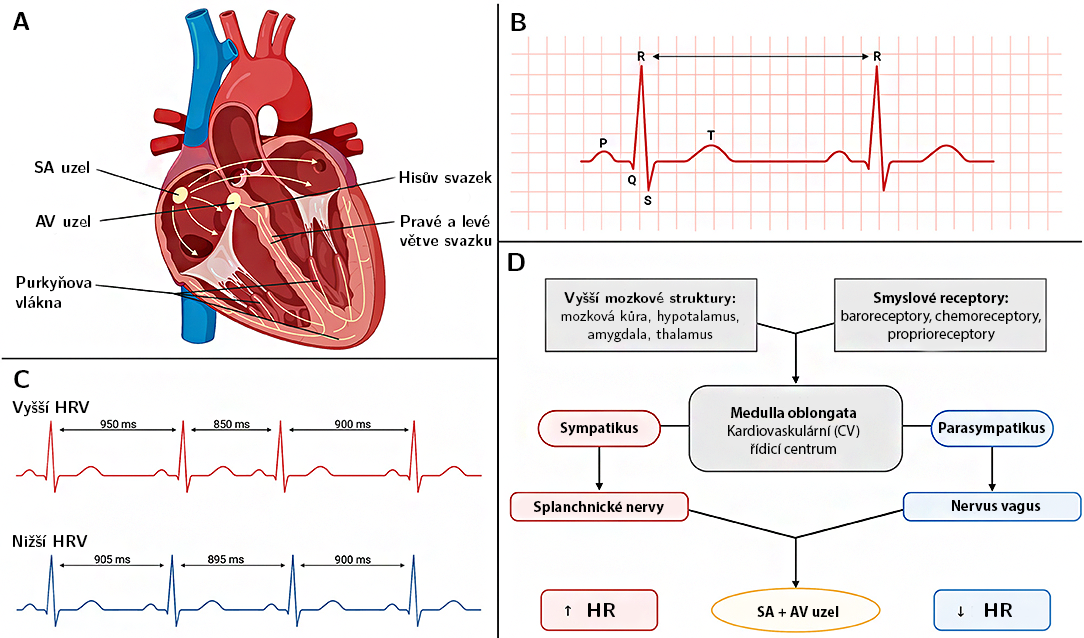
\includegraphics[width=1\linewidth]{figures/hrv_diagram}
        \caption{\textbf{(A)} Převodní systém srdeční; \textbf{(B)} Schéma
            \gls{EKG} záznamu elektrické aktivity; \textbf{(C)} Vysoká vs. nízká
            variabilita srdeční frekvence; \textbf{(D)} Schéma znázorňující
            různé faktory ovlivňující \gls{HR} a \gls{HRV} resp. zjednodušená
            část \gls{NVI} modelu (Upraveno a převzato z~\cite{Lujan2021})}
        \label{fig:hrv_diagram}
    \end{center}
\end{figure}

Jak již bylo řečeno, \gls{HRV} lze získat jako časovou diferenci mezi jednotlivými
srdečními údery, přičemž úder označujeme jako depolarizaci komor. To je část
srdečního cyklu, během které dochází ke genezi QRS komplexu. Aby bylo možné tuto
časovou diferenci vypočítat, je potřeba zmíněný komplex detekovat. K tomu se
využívá elektrokardiogram neboli záznam elektrické aktivity srdce, na kterém QRS
komplex představuje vývoj elektrické aktivace komor myokardu. Srdeční cyklus a
anatomie srdce již byly detailně popsány v~\cite{Stejfa2006,Weinhaus2005,Cihak2016}.
EKG záznam společně s QRS komplexem lze vidět na ilustraci~\ref{fig:hrv_diagram}B.

K detekci QRS komplexu se primárně využívá jeho pozitivní kmit neboli R vlna,
která se v \gls{EKG} signálu za fyziologických podmínek vyskytuje periodicky, v
závislosti na srdečním rytmu, konkrétně na autorytmických buňkách. Tyto srdeční
buňky generují stimulační elektrické potenciály, jež iniciují srdeční stah.
Hlavnimi dvěma iniciátory (pacemakerami), určující srdeční frekvenci, jsou
sinoatriální (\gls{SA}) a atrioventrikulární (\gls{AV}) uzel. Převodní systém
srdeční byl již podrobně popsán v~\cite{Stejfa2006,Weinhaus2005,Goldberger2017}
a lze vidět na Obr.~\ref{fig:hrv_diagram}A. Za účelem detekce samotné se využívá
mnoho algoritmů založených například na: vlnkové nebo Hilbertově transformaci,
prahování nebo neuronových sítích. Každý algoritmus zároveň samozřejmě využívá a
těží ze svého vlastního způsobu předzpracování EKG. Některé populární algoritmy
popsali Porr a Howell v~\cite{Porr2019}. Fluktuaci časových diferencí mezi po
sobě jdoucími R vlny a náležitou změnu HRV lze pozorovat na
Obr.~\ref{fig:hrv_diagram}C.

\subsection{Trendy v analýze HRV}
\label{subsec:hrv_analysis_trends}
Oblast vývoje problematiky analýzy variability srdečního rytmu je možné rozdělit
na několik podskupin. První podskupinu tvoří příznaky použité k analýze. Výběr
\gls{HRV} příznaků (parametrů) hraje významnou roli v rámci mapování vnějších
vlivů na funkci biosignálu. Z počátku se využívalo pouze deskriptivní statistiky
na řady nasbíraných hodnot srdečního rytmu pro účely odhalení srdečních
patologií. Zlom ale nastal v 70. letech 20. století, kdy se k analýze začaly
využívat R--R intervaly, a došlo tak k vývoji nových časových parametrů,
například \gls{RMSSD}, pNN50 nebo SDNN, které se stále hojně využívají. Poté
přišla na řadu spektrální a nelineární analýza, tedy frekvenční a nelineární
parametry, které sebou přinesli i nový vizuální nadhled. V poslední době se
používá hlavně časovo-frekvenční analýza, během které se aplikují spektrální
metody na specificky dlouhá časová okna a získají se tak frekvenční parametry
jako LF (Low Frequency) nebo HF (High Frequency). Je tak umožněno sledování
okamžitých změn \gls{HRV}, což může účinně diagnostikovat například
kardiovaskulární onemocnění~\cite{Shaffer2014,Ishaque2021}.

\begin{table}[h!]
    % \setlength{\tabcolsep}{10pt}
    \renewcommand{\arraystretch}{1.2}
    \scriptsize
    \centering
    \begin{threeparttable}
        \caption{Vybrané parametry z časové a frekvenční oblasti~\cite{Ishaque2021}}
        \label{tab:hrv_params}
        \begin{tabular}{p{2cm}p{12cm}}
            \toprule
            Parametr & Popis                                                                                                                                                        \\ \midrule
            SDNN     & Směrodatná odchylka intervalu mezi dvěma normálními srdečními tepy (NN). NN měří celkový výkon. Snižuje se v reakci na \gls{CL}                              \\
            RMSSD    & Střední kvadratická hodnota po sobě jdoucích rozdílů mezi normálními srdečními tepy. Primárně se řídí aktivitou \gls{PNS}                                    \\
            pNN50    & Vyjadřuje procento rozdílu spojeného s intervalem NN, který se liší o více než 50 ms. Korelaci s aktivitou \gls{PNS}, RMSSD, HF                              \\
            SD1      & Nelineární proměnné odvozené z Poincarého grafu. Sdílí vysokou korelaci s HF, RMSSD. Snižuje se v důsledku \gls{CL}                                          \\
            SD2      & Nelineární proměnné odvozené z Poincarého grafu. Sdílí vysokou korelaci s LF. Zvyšuje se v reakci na \gls{CL}                                                \\
            GSR std  & Směrodatná odchylka spojená s elektrodermální aktivitou. Zvyšuje se během \gls{CL}                                                                           \\
            GSR mean & Průměrná hodnota získaná měřením rychlosti změn spojených s aktivitou EDA. Zvyšuje se během \gls{CL}                                                         \\
            RSP rate & Představuje frekvenci dýchání, zvýšení respirační frekvence vede ke zvýšení aktivity \gls{PNS}, VF a snížení LF a aktivity SNS. Zvýšení v reakci na \gls{CL} \\
            LF       & Reprezentuje 0,04--0,15 Hz v rámci PSD\tnote{1} ~a většinou se používá k označení aktivity \gls{SNS} ale může specifikovat i aktivitu \gls{PNS}              \\
            HF       & Představuje frekvenční rozsah 0,15--0,40 Hz a označuje výhradně aktivitu \gls{PNS}                                                                           \\ \bottomrule
        \end{tabular}
        \begin{tablenotes}
            \item [1] Výkonová spektrální hustota (anglicky Power Spectral
            Density) --- vyjadřuje výkon obsažený v určitém intervalu spojitého
            frekvenčního spektra
        \end{tablenotes}
    \end{threeparttable}
\end{table}

Do další podskupiny lze zařadit způsoby měření \gls{HRV}. Od 90. let 20. století
se výzkum \gls{HRV} rozšířil o analýzu využitím krevního tlaku a dýchání
prostřednictvím fotopletysmografie (\gls{PPG}) a hrudních pásů. Došlo tak k
prohloubení HRV výzkumu vzhledem k multimodálnímu přístupu měření. Od roku 2000
se využitím dvanáctisvodového EKG začali v klinické praxi efektivněji analyzovat
srdeční patologie. Současně se využívá nositelných technologií (tzv. wearables)
v podobě například hodinek na zápěstí, které však často měřené parametry
poskytují pouze agregovaně za určité časové úseky. Výhodou je sice jejich
mobilita ale na úkor přesnosti poskytovaných dat. Detailní popis zmíněných
podskupin společně s dalšími trendy byl již uveden v~\cite{Ishaque2021}.

\subsection{Struktura HRV indexů}
\label{subsec:hrv_indices}
Vzhledem k popularitě analýzy \gls{HRV} napříč obory vznikla problematika
týkající se interpretace dostupných metrik. Jedním z hlavních problémů je tedy
nedostatečné pochopení funkčního vztahu mezi \gls{HRV} ukazateli a
fyziologickými procesy. Také se tyto ukazatele často používají zaměnitelně, což
jen přispívá k nejasnostem ohledně jejich skutečného významu
(funkce)~\cite{Fatisson2016,hayano2019}. Zároveň se často \gls{HRV} metriky
používají kombinovaně. To představuje několik problémů při interpretaci výsledků
výzkumu a může být příčinou nekonzistentních výsledků. Dalším problémem je
reprodukovatelnost, jelikož různé studie zkoumající stejný jev mohou při popisu
vztahu s variabilitou srdeční frekvence vycházet z různých ukazatelů. Také se
často nebere ohled na podobnost a překrývání mnoha těchto ukazatelů. Studie
například ukázaly, že indexy v časové a frekvenční oblasti, jako je RMSSD a
pNN50, spolu silně korelují a jsou vysoce spojeny s výkonem HF. V důsledku toho
lze tyto míry považovat za zaměnitelné při hodnocení parasympatické modulace
\gls{HRV}. Nejasnosti ohledně fyziologických důsledků těchto ukazatelů zvyšují
právě náročnost objasnění jejich
výsledků~\cite{Bigger1989,Rohila2020,Malik1996,Ishaque2021}.

Je také třeba poznamenat, že výpočet RMSSD zahrnuje výpočet rozdílů mezi po sobě
jdoucími R--R (N--N) intervaly. V důsledku toho tento index odráží především
vysokofrekvenční oscilační vzorce srdečního rytmu a není ovlivněn dlouhodobými
změnami. Naproti tomu SDNN, o němž se předpokládá, že zachycuje jak sympatickou,
tak parasympatickou aktivitu, je silně spojen s celkovým výkonem ve výkonovém
spektru \gls{HRV}~\cite{Bigger1989,Malik1996,Ishaque2021,Acharya2006}.

V posledních letech se parametry SD1 a SD2 konvenčně interpretují jako
nelineární. Toto tvrzeni bylo však znehodnoceno matematickým důkazem, který
potvrdil, že metriky RMSSD a SD1 jsou ekvivalentní. Tím pádem studie, které
uvádějí tyto dva krátkodobé \gls{HRV} indexy často vágně dospívají k podobným
statistickým výsledkům, aniž by tuto ekvivalenci
rozpoznaly~\cite{Ciccone2017,Tam2021,Leite2015,Rohila2020,Peng2015}.

Některé studie navíc zaznamenaly podobnosti mezi poměrovými parametry SD1/SD2 a
LF/HF při hodnocení rovnováhy mezi krátkodobou a dlouhodobou variabilitou
srdečního rytmu. Nezohlednění těchto překryvů v analýzách může vést ke
statistickým chybám. Ty mohou zahrnovat přílišnou důvěru v závěry (projevující
se falešně vysokým počtem parametrů shodujících se s určitým trendem), problémy
s kolinearitou (pokud je jako prediktory použito více metrik současně),
potenciální nadměrnou korekci (např. prostřednictvím metod úpravy p-hodnoty
Bonferroniho typu) a zbytečnou složitost
výsledků~\cite{Tam2021,Rohila2020,Dormman2013,Guzik2013,Brennan2002}.


\section{Periferní biosignály}
\label{sec:peripheral_biosignals}
Včetně elektrické srdeční aktivity, která byla diskutována v minulé sekci a je
hlavní zkoumanou proměnnou, se mezi další periferní biosignály zkoumané v této
práci řadí také elektrodermální a respirační aktivita. V následující podkapitole
jsou tyto periferní biosignály uvedeny do souvislosti s problematikou práce a
předchozími kapitolami. Dále je stručný přehled jak lze zkoumané signály
zaznamenat a zpracovat.

O elektrodermální aktivitě lze hovořit jako o fyziologickém procesu, úzce
spojeném s aktivitou potních žláz v kůži, jež je ovlivňován \gls{ANS}. Aktivita
potních žláz vede ke změnám elektrického odporu kůže. Zvýšením této aktivity tak
dochází k poklesu elektrického odporu kůže (zvýšení kožní vodivosti) a
naopak~\cite{Boucsein2012,Critchley2002,Tronstad2022}. Fredrikson et
al.~\cite{Fredrikson1998} ukázali, že EDA je úzce spojená s aktivitou cingulární
kůry, sekundární zrakové kůry a pravé inferiorní parietální kůry, přičemž
nejsilnější korelace byla pozorována v pravé insulární kůře, která je součástí
\gls{CAN}. Další studie naznačují mnohočetné souvislosti mezi změnami kožní
vodivosti a \gls{CAN} regiony~\cite{Critchley2002,Buchwald2019,Caruelle2019,Sanchez2020}.
EDA tedy nachází velké uplatnění v neuropsychofyziologickém výzkumu ale stejně jako u HRV
se zde vyskytují problémy s interpretací metrik, které z ní
vycházejí~\cite{Blechert2016}. Z anatomického, fyziologického a biofyzikálního
hlediska byla již elektrodermální aktivita důkladně rozebrána v~\cite{Boucsein2012}.
Úzkou provázanost kožní vodivosti a kognitivní zátěže s využitím EDA pro její detekci
a hodnocení podkládají studie~\cite{Bahauddin2021,Ghaderyan2018,Hossain2019,
    Nourbakhsh2012,Paas2003,Posada2018,Shi2007,Shimomura2008}.

Respirační aktivitou se rozumí proces dýchání, při kterém dochází k výměně
kyslíku a oxidu uhličitého mezi plícemi a okolím. Dýchací ústrojí bylo již
důkladně popsáno v~\cite{Kara2010}. Respirační signál jako takový odráží
cyklické změny objemu plic během dýchání. Dýchací aktivita je ovlivněna celou
řadou faktorů, včetně fyzické aktivity, stresu, emocí a i kognitivních nároků.
Například kognitivní úkoly vyžadující trvalou pozornost nebo vyšší nároky na
pracovní paměť mohou zvýšit dechovou námahu a spotřebu kyslíku v mozku. Obecně
se amplituda a frekvence dechového signálu zvyšuje s rostoucí kognitivní
zátěží~\cite{Ayres2021}. Existuje mnoho studií, které vypovídají o významném
vztahu mezi respiračním signálem a \gls{CL}, avšak oproti srdeční a
elektrodermální aktivitě je tento signál mnohem častěji zanedbáván. To může
vysvětlovat větší počet protichůdných a negativních studií, které popírají
význam RSP při detekci a hodnocení kognitivní
zátěže~\cite{Ayres2021,Grassmann2016}.

\subsection{Měření biosignálů}
\label{subsec:srdecni_aktivita}
V následujících sekcích jsou popsany principy měření a postupy zpracování
periferních biosignálu, které byly využívány pro účely této diplomové práce.
Těmi jsou konkrétně srdeční, elektrodermální a respirační aktivita.

\subsubsection{Elektrická srdeční aktivita}
Záznam elektrické srdeční aktivity (elektrokardiogram) je výstupem komplexních
fyziologických a technologických procesů. Z fyziologického hlediska je třeba
nahlédnout na celulární úroveň, kde díky toku iontů přes buněčné membrány a mezi
sousedními buňkami vznikají transmembránové iontové proudy. Geneze těchto proudů
je synchronizována díky srdečnímu cyklu, během kterého dochází k tvorbě časově
závislého elektrické pole v myokardu. Toto elektrické pole pak podléhá
interferenci různých dalších struktur, jako jsou plíce, krev a kosterní svalstvo
až kůže. Na kůži jsou poté proudy detekovány elektrodami umístěnými na určitých
místech končetin a trupu v takové konfiguraci, aby vytvářely svody, konkrétně
bipolární svody~\cite{mirvis2001}. Elektrofyziologie myokardu byla již detailně
popsána v~\cite{Goldberger2017,Cihak2016,Stejfa2006,Weinhaus2005}.

Svody zaznamenávají rozdíl potenciálů mezi dvěma elektrodami, přičemž jedna je
označována jako kladná a druhá záporná. Bipolární potenciál se následně získává
jako rozdíl potenciálů kladné a záporné elektrody. U některých konfigurací je
elektricky spojeno více elektrod, které představují záporný člen bipolárního
páru, označovaný jako referenční elektroda. Výstupní potenciály elektrod jsou ve
finále zesíleny, filtrovány~\cite{Goldberger2017,mirvis2001}.

Jednou z konfigurací je standardní klinické EKG, které zahrnuje záznamy z 12
svodů. Svody v tomto případě sestávají ze standardních končetinových svodů
(svody I, II a III), šesti prekordiálních svodů (svody V1 až V6) a ze tří
rozšířených (augmentovaných) končetinových svodů\footnote{Prekordiální a
    rozšířené končetinové elektrody jsou často označované jako \enquote{unipolární}
    svody.} (svody aVR, aVL a aVF)~\cite{Goldberger2017,mirvis2001}.

\begin{figure}[htb!]
    \begin{center}
        \includegraphics[width=1\linewidth]{figures/ecg_leads}
        \caption{Ilustrace 12svodového EKG systému. \textbf{A)} Prostorové
            rozmístění 10 elektrod: tři končetinové svody, tři rozšířené končetinové
            svody a šest prekordiálních (hrudních) svodů, které byly vytvořeny mezi
            fyzickými elektrodami a virtuální elektrodou známou jako Wilsonův
            centrální terminál ($V_W$). \textbf{B)} Rozdíly elektrických potenciálů
            mezi elektrodami odrážejí elektrickou aktivitu srdce z různých
            prostorových úhlů~(Přeloženo a převzato z~\cite{Yao2020})}
        \label{fig:ecg_leads}
    \end{center}
\end{figure}

\paragraph{Standardní končetinové svody.}
Standardní končetinové svody zachycují rozdíly potenciálů mezi dvěma
končetinami. Elektroda na pravé noze slouží jako referenční, snižuje šum a není
tak součástí konfigurace svodů. Svody jsou uspořádány do trojúhelníku, který se
často nazývá jako Einthovenův trojúhelník. Toto uspořádání zajišťuje, že
potenciál snímaný ve svodu II odpovídá součtu potenciálů měřených ve svodech I a
III~\cite{Goldberger2017,mirvis2001}.

\paragraph{Prekordiální svody a wilsonův centrální terminál.}
Prekordiální svody se používají k záznamu potenciálu v každém ze šesti určených
míst trupu vzhledem k referenci. Na každé místo se umístí aktivní elektroda
připojená ke kladnému vstupu záznamového systému. Referenčním vstupem je složená
elektroda známá jako Wilsonova centrální svorka, která je vytvořena kombinací
výstupu elektrod levé paže (LA), pravé paže (RA) a levé nohy (LL)
prostřednictvím odporů (5000~\si{\ohm})~\cite{Goldberger2017,mirvis2001}.

\paragraph{Rozšířené končetinové svody.}
Jak již bylo zmíněno, třemi augmentovanými svody jsou aVR, aVL a aVF. U svodu
aVR je aktivní elektrodou sloužící jako pozitivní vstup elektroda pravé paže,
zatímco u svodu aVL je to elektroda levé paže a u svodu aVF elektroda levé nohy.
Referenční potenciál je zde vytvořen spojením dvou končetinových elektrod, které
se nepoužívají jako aktivní. Účelem tohoto modifikovaného referenčního systému
je generovat signál s vyšší amplitudou než při použití Wilsonovy centrální
svorky jako referenční elektrody~\cite{Goldberger2017,mirvis2001}.

\paragraph{Další svodové systémy.}
Byly vyvinuty různé svodové systémy, které umožňují detekovat diagnosticky
významné informace, jež nemusí být zachyceny standardním 12svodovým EKG, a
zlepšit efektivitu záznamu, přenosu a ukládání EKG. Používají se například levé
zadní svody k detekci akutních posterolaterálních infarktů nebo elektrodová pole
o 80 nebo více elektrodách k zobrazení potenciálů povrchu těla jako izopotenciálních
map~\cite{Goldberger2017,mirvis2001}. Přehled dalších svodových systému včetně
nositelných byl popsán v~\cite{Baig2013,Majumder2018,Serhani2020}.

\subsubsection{Elektrodermální aktivita}
V úvodu kapitoly bylo řečeno, že princip měření EDA je založen na skutečnosti,
že činnost potních žláz v kůži, která je regulována sympatickým nervovým
systémem, vede ke změnám vodivosti kůže. Díky tomu, a jak může vyplývat z
minulých kapitol, je měření EDA běžně používanou metodou pro hodnocení
fyziologických reakcí souvisejících s emočními a kognitivními procesy.

\begin{figure}[htb!]
    \begin{center}
        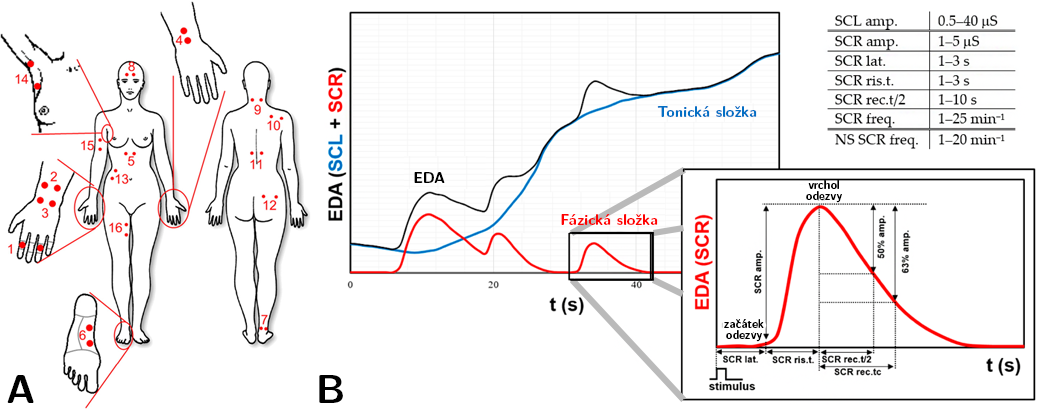
\includegraphics[width=1\linewidth]{figures/EDA}
        \caption{\textbf{A)} Možná místa měření kožní vodivosti. \textbf{B)}
            Typická odezva elektrodermální aktivity~(Upraveno a převzato
            z~\cite{Janssen2012,Vavrinsky2021})}
        \label{fig:eda_mereni}
    \end{center}
\end{figure}

Měření elektrodermální aktivity zahrnuje umístění dvou elektrod na kůži, přičemž
jedna měří rozdíly potenciálů mezi dvěma body na kůži a druhá slouží jako
referenční elektroda. Elektrody se obvykle umísťují na prsty nebo dlaň ruky, i
když lze použít i jiná místa, například chodidla nebo čelo (viz
Obr.~\ref{fig:eda_mereni}A) a měří se elektrická vodivost kůže v reakci na malý
stejnosměrný nebo střídavý proud proud~\cite{Caruelle2019,Boucsein2012}.

Z pohledu způsobu měření elektrodermální aktivity lze tedy rozlišovat dvě hlavní
kategorie: endosomatická a exosomatická měření. V rámci endosomatického měření
se zaznamenává pouze potenciál generovaný kůží bez použití vnějšího zdroje. U
exosomatického měření se využívají externí zdroje, jako je právě střídavý nebo
stejnosměrný proud přiváděný na kůži. Aplikace konstantního stejnosměrného
napětí nebo proudu umožňuje měření vodivosti kůže (resp. odporu kůže podle
Ohmova zákona). Pokud se ale aplikuje konstantní střídavé napětí nebo proud, tak
lze měřit kožní admitanci (resp. kožní impedanci). Nejpoužívanější metodou pro
exosomatická měření je metoda stejnosměrného konstantního napětí, a to primárně
díky jednoduššímu procesu vyhodnocování a interpretace než je tomu tak u
endosomatického způsobu~\cite{Boucsein2012,Li2022,Posada2020,Caruelle2019}.

Měřená kožní vodivost nebo kožní potenciál se vyjadřují v jednotkách vodivosti
(mikrosiemens, \si{\micro\siemens}) a napětí (\si{\milli\volt}). V naměřeném
signálu se odrážejí změny v různých časových škálách, které se běžně dělí na dvě
složky: tonickou (\gls{SCL}) a fázickou (\gls{SCR}). Tonická složka představuje
velikost kožní vodivosti nebo potenciálu v nepřítomnosti sudomotorické nervové
aktivity\footnote{Sudomotorická nervová aktivita se vztahuje k \gls{ANS}
    kontrole aktivity potních žláz v reakci na různé environmentální a individuální
    faktory.}, zatímco ta fázická se týká rychlých změn kožní vodivosti nebo
potenciálu jako přímého důsledku sudomotorického vzruchu. Fázická složka je
charakterizován nástupem (SCR ris.), dobou nárůstu (SCR ris. t.), amplitudou
(SCR amp.) a dobou zotavení (SCR rec. tc.). Na Obr.~\ref{fig:eda_mereni} lze
vidět průběh EDA složek společně s jejich korespondujícím popisem. Tonické a
fázické složky lze oddělit pomocí technik zpracování
signálu~\cite{Boucsein2012,Li2022,Posada2020,Caruelle2019,Caruelle2019}.

\subsubsection{Respirační aktivita}
\label{subsec:respiracni_aktivita}
Pro měření dechové aktivity (resp. dechové frekvence) je k dispozici mnoho
metod, od přímého měření ventilace až po nepřímé měření pohybů souvisejících s
dýcháním. V této sekci je stručný přehled často používaných metod měření dechové
aktivity.

\begin{figure}[htb!]
    \begin{center}
        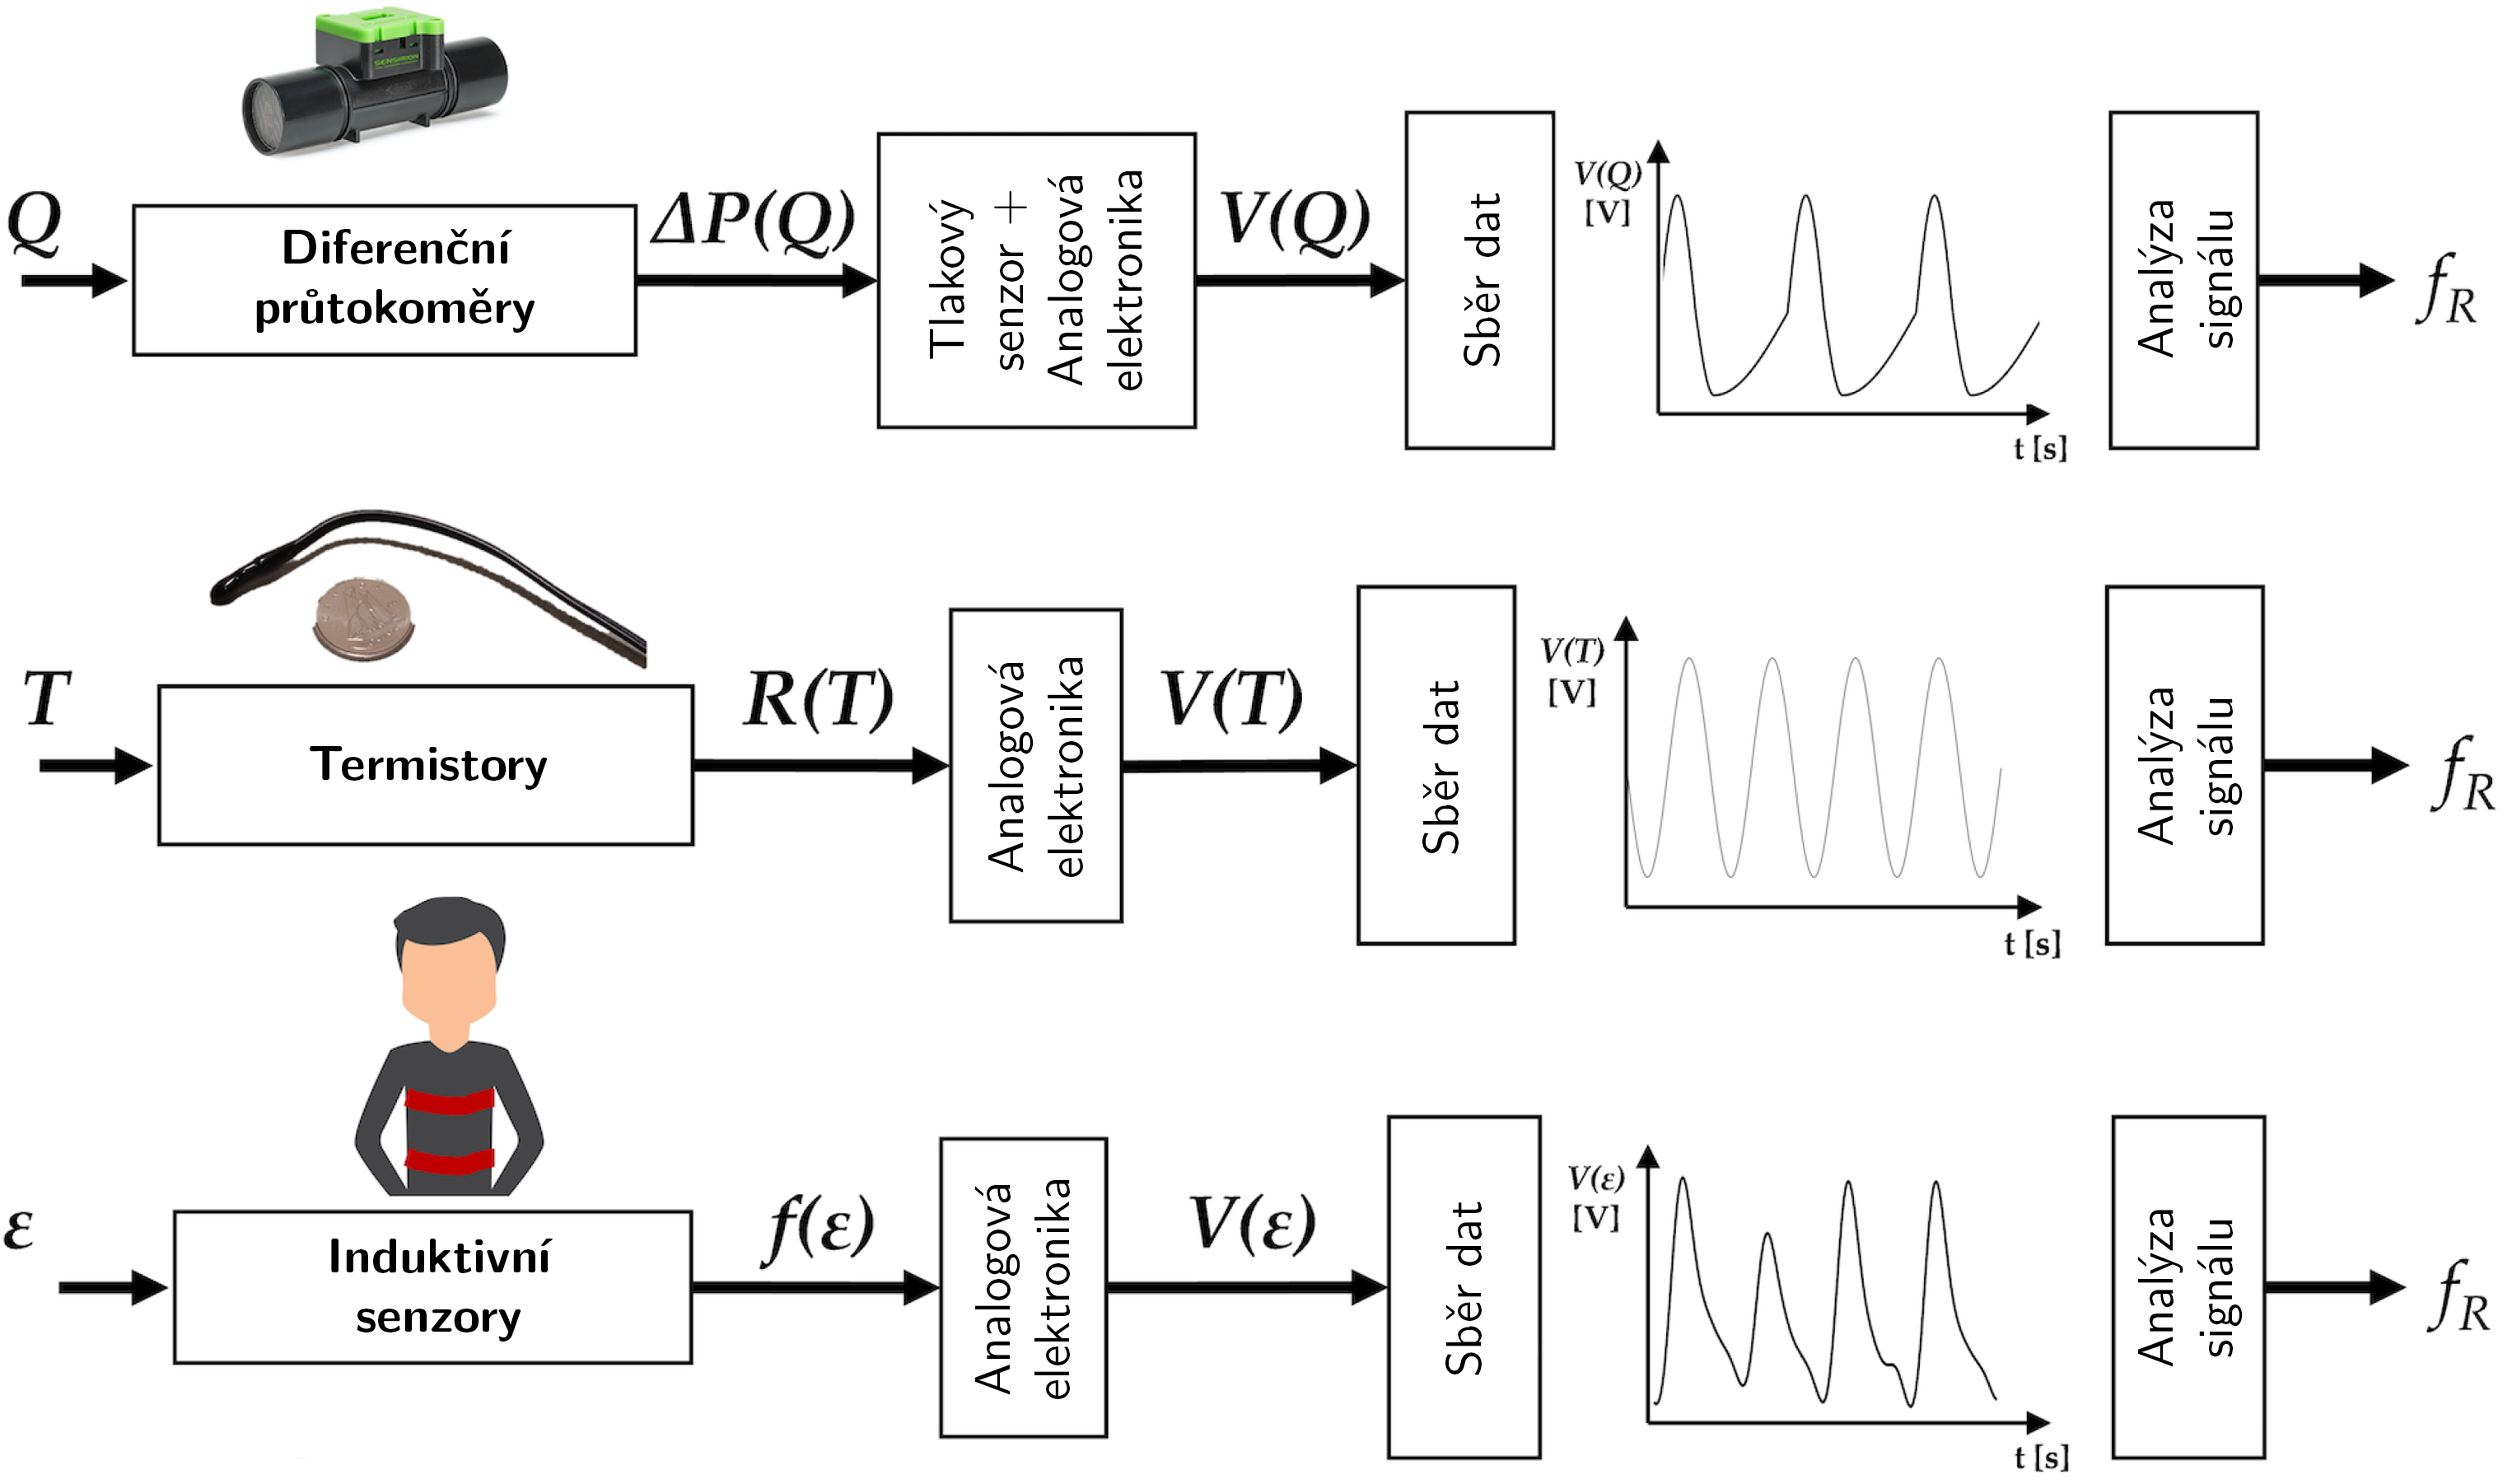
\includegraphics[width=1\linewidth]{figures/rsp_measure}
        \caption{Různé technologie pro měření dechové frekvence ($f_R$). Nahoře
        z kategorie snímačů proudění vzduchu, kde $ΔP(Q)$ je změna úbytku tlaku
        způsobená prouděním vzduchu $Q$. Uprostřed z kategorie snímačů teploty,
        kde $R(T)$ je změna odporu způsobená vlivem teploty $T$. Dole z
        kategorie tenzometrických snímačů, kde $f(\mathcal{E})$ je změna odporu
        způsobená deformačním tlakem $\mathcal{E}$. $V(X)$ je výstupní
        napětí~(Upraveno a převzato z~\cite{Massaroni2019})}
        \label{fig:rsp_mereni}
    \end{center}
\end{figure}

Jednou z nejběžnějších metod měření dechové aktivity je přímé měření ventilace.
Ventilace je celkový objem vzduchu, který se během každého nádechu přesune do
plic a z plic ven, a lze ji měřit pomocí několika technik včetně spirometrie,
pletysmografie, a kapnometrie. Spirometrie měří objem vzduchu, který je
vdechován a vydechován, zatímco pletysmografie měří změny tlaku v uzavřené
komoře během dýchání. Kapnometrie měří koncentraci oxidu uhličitého ve
vydechovaném vzduchu, což úzce souvisí s ventilací. Tyto techniky umožňují
přesné měření dechové aktivity, ale mohou být invazivní a vyžadují
specializované vybavení~\cite{Massaroni2019,Massaroni2021,Liu2019}. 

Alternativní metodou měření dechové aktivity je nepřímé měření pohybů
souvisejících s dýcháním. Tyto pohyby lze detekovat pomocí senzorů umístěných na
hrudníku nebo břiše, jako jsou piezoelektrické senzory, tenzometry nebo
akcelerometry. Tyto snímače detekují změny tvaru nebo pohybu hrudníku nebo
břicha během dýchání a lze je použít k odhadu dechové frekvence a objemu. Tyto
metody jsou méně invazivní než přímé měření ventilace a lze je použít v reálném
prostředí, avšak u některých populací nebo za určitých podmínek mohou být méně
přesné~\cite{Massaroni2019,Massaroni2021,Fazio2021,Liu2019}.

Další nově se objevující metodou měření dechové aktivity je používání
nositelných zařízení, jako jsou chytré hodinky, které mohou detekovat změny
dechových vzorců pomocí fotopletysmografie nebo akcelerometrie.
Fotopletysmografie měří změny objemu krve pomocí světelných senzorů, zatímco
akcelerometrie měří pohyb pomocí pohybových senzorů. Tyto metody jsou
neinvazivní a lze je použít v přirozeném prostředí s tím, že mohou být omezené
ve své přesnosti a preciznosti~\cite{Massaroni2019,Massaroni2021,Fazio2021,
Leube2020,Liu2019,Nam2022,Zschocke2022}. 

\subsection{Postupy zpracování biosignálů}
\label{subsec:postupy_zpracovani_biosignalu}
Zpracování biosignálů označuje techniky a postupy používané k získání informací
z biosignálů, ke zvýšení jejich kvality a k interpretaci jejich významu. V této
sekci je uveden přehled hlavních postupů zpracování biosignálů, včetně jejich
akvizice, předzpracování, extrakce příznaků a klasifikace. 

Sběr signálu znamená proces záznamu biosignálů z lidského těla pomocí měřicích
zařízení, jako jsou senzory nebo elektrody. Kvalita zaznamenaných signálů závisí
na různých faktorech, jako je typ a umístění snímačů, odstup signálu od šumu a
vzorkovací frekvence. Například signály EKG se zaznamenávají pomocí elektrod a
jejich umístění ovlivňuje kvalitu zaznamenaných signálů, protože různé oblasti
srdce mohou mít různou sílu nebo frekvenci signálu. Kromě toho se odstup signálu
od šumu týká poměru žádoucího signálu a nežádoucího šumu v zaznamenaných
signálech. Čím vyšší je poměr signál/šum, tím jsou zaznamenané signály jasnější
a spolehlivější. A konečně vzorkovací frekvence označuje frekvenci, s jakou jsou
signály vzorkovány nebo digitalizovány. Čím vyšší je vzorkovací frekvence, tím
přesnější je digitální reprezentace signálů~\cite{Escabi2005,Karagiannis2011}.

\begin{figure}[htb!]
    \begin{center}
        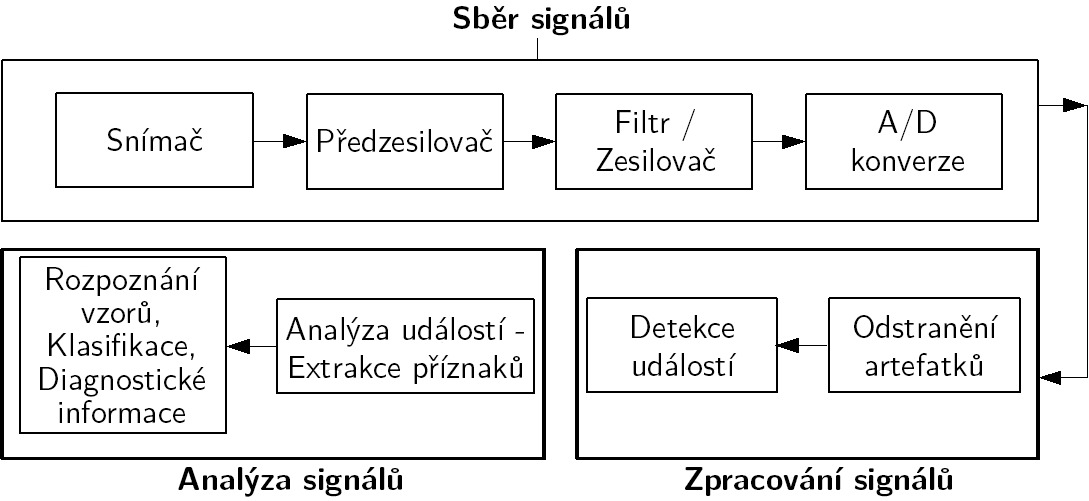
\includegraphics[width=1\linewidth]{figures/signal_processing_diagram}
        \caption{Řetězec procesů od získání biomedicínského signálu po fázi
        analýzy~(Přeloženo a převzato z~\cite{Karagiannis2011})}
        \label{fig:zpracovani_biosignalu_diagram}
    \end{center}
\end{figure}

Předzpracování se týká postupů používaných k přípravě zaznamenaných signálů pro
další analýzu. Mezi postupy předzpracování patří především filtrování signálu.
Žádoucí je často navržení takového filtru, který rovnou koriguje kolísání nulové
izolinie a potlačuje nežádoucí artefakty (síťový šum, svalové artefakty, apod.).
V některých případech však nestačí pouze frekvenčně selektivní filtrace a volí
se jiné přístupy. Zvolený přístup závisí na zdroji a charakteru signálu.
Porovnání metod předzpracování srdeční, elektrodermální a respirační aktivity
bylo vypracováno v ~\cite{Escabi2005,Khodadad2018,Power2020,Subramanian2019}. 

Extrakce příznaků označuje postupy používané k extrakci relevantních informací
nebo charakteristik z předzpracovaných signálů. Extrakce příznaků je důležitým
krokem při zpracování biosignálů, protože jednak snižuje dimenzionalitu signálů
a také zvýrazňuje právě relevantní informace. Z biosignálů lze extrahovat různé
typy příznaků, například z časové, z frekvenční nebo nelineární
oblasti~\cite{Escabi2005,Karagiannis2011}. Krishnan a Athavale popsali trendy v
extrakci příznaků biomedicínských signálů v~\cite{Krishnan2018}.

Klasifikací se rozumí postupy používané k přiřazení značky (anotace) nebo
kategorie biosignálu na základě jeho extrahovaných vlastností (příznaků).
Klasifikace je dalším důležitým krokem při zpracování biosignálů, protože
umožňuje identifikovat vzory nebo trendy v signálech a předpovídat fyziologický
stav nebo kondici subjektu~\cite{Escabi2005,Karagiannis2011}. Možnosti využití
klasifikace (resp. metod strojového učení) pro biomedicínské aplikace byly
popsány v~\cite{Foster2014,Kording2018,Strzelecki2022}.

Zpracování biosignálů se potýká s různými problémy a omezeními, jako je
variabilita signálů, složitost postupů zpracování a interpretace výsledků.
Variabilitou signálů je myšleno, že biosignály se mohou lišit od subjektu k
subjektu, od sezení k sezení nebo dokonce v rámci jednoho sezení. Tato
variabilita může ovlivnit kvalitu a spolehlivost zaznamenaných signálů a může
vyžadovat použití sofistikovanějších metod předzpracování a
klasifikaci~\cite{Escabi2005,Karagiannis2011}.

\section{Strojové učení}
\label{sec:machine_learning}
Strojové učení (anglicky Machine Learning, \gls{ML}) představuje odvětví umělé
inteligence, které se zaměřuje na vytváření matematických modelů a zvyšování
jejich přesnosti predikce na základě předchozích zkušeností. Tyto zkušenosti se
získávají retrospektivně z dostupných dat (trénovacích dat), která se využívají
k formulaci pravidel a identifikaci charakteristických rysů nebo vztahů v
datech. Proces učení zahrnuje techniky, které vyplývají z  oborů informatiky,
statistiky, pravděpodobnosti nebo optimalizace. Využití algoritmů strojového
učení se neustále rozšiřuje v mnoha oblastech díky rostoucí dostupnosti online
dat a snižování nákladů na výpočetní zdroje. Rozsah oblastí použití zahrnuje
široké spektrum oborů, včetně zdravotnictví.

Tato kapitola slouží jako úvod do vybraných základních pojmů strojového učení s
cílem vytvořit teoretický náhled pro podporu pochopení problematiky v
korespondujících částech práce. Detailněji byly principy a náležitosti
strojového učení již popsány v
literatuře~\cite{Aurelien2022,Murphy2012,Goodfellow2016}.

\subsection{Typy systémů strojového učení}
Různorodost scénářů strojového učení je charakterizována rozdíly v povaze
trénovacích dat, způsobem trénování a kritérii hodnocení. Každý přístup je
vhodný pro řešení určité kategorie problémů a představuje své vlastní
charakteristické výhody a omezení. V následujících podkapitolách jsou rozebrány
primárně dvě nejrozšířenější formy přístupů k učení, tj. učení s učitelem
(anglicky Supervised Learning) a učení bez učitele (anglicky Unsupervised
Learning).

\subsubsection{Učení s učitelem}
\label{subsubsec:supervised_learning}
Učení s učitelem je typ strojového učení, během kterého se využívají právě
taková trénovací data, která mají anotovanou výstupní proměnnou. Úkolem je zde
aproximovat mapovací funkci $h$, která predikuje výstupní proměnnou na základě
vstupní proměnné $X$. K aproximaci mapovací funkce jsou použita označená
trénovací data, která se skládají z $n$ párů vstupních a výstupních proměnných.
Cílem je získat přesné predikce jak pro trénovací, tak pro úplně nová data.
Formálně lze tedy tvrdit, že hledáme zobrazení:
\begin{equation}
    h:\mathbb{R}^d \rightarrow \mathcal{C}
\end{equation}
tak, že pro každou novou dvojici vstupu a výstupu $(x,y)$ vybranou z
$\mathcal{P}$ platí $h(X) ≈ y$, kde $\mathbb{R}^d$ je $d$-rozměrný příznakový
prostor a $\mathcal{C}$ je prostor všech možných tříd. Zároveň předpokládáme, že
tyto dvojice pocházejí z neznámého rozdělení $\mathcal{P}$~\cite{Murphy2012}.

\subsubsection{Učení bez učitele}
Cílem učení bez učitele je najít vzory v neanotovaných datech bez definovaného
výstupu. Výsledkem tohoto typu učení mohou být struktury nebo vztahy v datech.
Vyhodnocování výkonu natrénovaného modelu je v tomto případě, bez označených
dat, často náročné. Běžnou úlohou pro tento typ učení je shlukování, které
seskupuje podobná data do shluků. Shlukování se používá například pro segmentaci
obrazových dat a provádí se pomocí algoritmů, jako je hustotní prostorové
shlukování (\gls{DBSCAN}), k-means nebo hierarchické shlukování.

\begin{figure}[!htb]
    \begin{center}
        \begin{tikzpicture}[board/.style={minimum width=6em,minimum height=1em,
                        draw,fill=gray!20,path picture={
                                \foreach \XX in {0,...,5}
                                    {\ifnum\XX>0
                                            \draw ([xshift=\XX*1em]path picture bounding box.north west)
                                            -- ([xshift=\XX*1em]path picture bounding box.south west);
                                        \fi
                                        \ifnum\XX=#1
                                            \draw[fill=blue!50] ([xshift=\XX*1em]path picture bounding box.north west)
                                            rectangle ([xshift=\XX*1em-1em]path picture bounding box.south west);
                                        \fi}
                            },pin={[name=pin-#1]right:Vyhodnocení$_{#1}$},scale=1.2},
                box/.style={draw,minimum size=1.2em,fill=blue!50,label={[node
                                        font=\tiny,align=center]#1}},
                2box/.style={rectangle split, rectangle split parts=2, draw,minimum
                        width=#1}, 2ell/.style={ellipse split,draw},
                every pin edge/.style={-stealth},font=\sffamily]
            \matrix[matrix of nodes,nodes in empty cells,nodes={anchor=center},
            row sep=1ex,column sep=1em,inner xsep=0.3em] (m) {
            1. & |[board=1]| \\
            2. & |[board=2]| \\
            3. & |[board=3]| \\
            4. & |[board=4]| \\
            5. & |[board=5]| \\
            };
            \draw[semithick,decorate,decoration={brace,mirror,raise=1pt}] (m-1-2.north east)
            -- ++ (-4.8em,0)
            node[midway,above=1ex,align=center] (TF) {Trénovací\\ vzorek};
            \node[left=1em of TF,align=center] (VF) {Validační\\ vzorek};
            \node[anchor=south,rotate=90] at (m.west){$k$-iterace};
            \draw (VF) -- ([xshift=0.6em]m-1-2.north west);
            \draw[semithick,decorate,decoration={brace,mirror,raise=1pt}] (m-5-2.south west) -- ++ (4.8em,0)
            coordinate[midway,below=1ex](5f);
            \draw[semithick,decorate,decoration={brace,raise=1pt}] (m.north east)
            -- (m.south east)  node[midway,right=1ex,2box=4em,draw=none,anchor=text west,
                rectangle split part align={left}]{Vyhodnocení
                \nodepart{two}$=\sum\limits_{i=1}^5\textsf{Vyhodnocení}_i$};
            \node[below=2em of m-5-2.south west,2box,fill=gray!20] (2box) {Trénovací vzorek\nodepart{two}Značky trénovacího vzorku};
            \node[below=2em of 2box,2ell,inner ysep=-0.2ex] (2ell){
                \begin{tabular}{@{}c@{}}
                    Hodnoty \\ hyperparametrů
                \end{tabular}
                \nodepart{lower}
                \begin{tabular}{@{}c@{}}
                    \textbf{Vybraný algortimus} \\
                    \textbf{strojového učení}
                \end{tabular}};
            \node[below=2em of 2ell,regular polygon,regular polygon
                sides=6,fill,text=white] (6gon) {Model};
            \draw[>=stealth]  (5f) edge[->] (2box) (2box) edge[->] (2ell) (2ell) edge[->] (6gon);
            %
            \draw[semithick,decorate,decoration={brace,mirror,raise=1pt}]
            (pin-5.south west) -- (pin-5.south east) coordinate[midway,below=1.2ex] (pf)
            node[midway,below=2em,box=left:{Validační\\ vzorek}](b1){};
            \node[right=4em of b1,box=above:Predikce,yshift=-0.5ex] (b2){};
            \node[below=4em of b2,box=below:{Validační\\ značky}] (b3){};
            \path (b2) -- (b3) coordinate[midway,right=1em] (aux)
            node[right=1em of aux] (PF) {Vyhodnocení};
            \draw[-stealth] (b2.east) -| (aux) |- (b3.east) (aux) -- (PF);
            \node[below=0.5em of b1,regular polygon,regular polygon sides=6,fill,text=white] (6gon2) {Model};
            \path coordinate[left=1em of b2] (aux2);
            \draw[-stealth] (6gon2.east) -| (aux2) |- (b1.east) (aux2) -- (b2);
            \draw[-stealth] (pf) -- (b1);
        \end{tikzpicture}
        \caption{Obecné schéma procesu trénování modelu a optimalizací
            hyperparametrů s využitím k-násobné křížové
            validace~\cite{crossvalidation}}
        \label{fig:cross-validation}
    \end{center}
\end{figure}


\subsection{Trénování a testování modelů}
Vyhodnocování modelů strojového učení je pro jejich úspěšnost klíčové. Aby bylo
zajištěno, že model dokáže efektivně predikovat i nová data, nikoli pouze data
využitá během jeho trénování, provádí se tzv. \emph{train-test} rozdělení. To
zahrnuje ponechání části dat jako testovací množiny, kterou model během
trénování nepoužil, a její následné použití k vyhodnocení schopnosti modelu
generalizace porovnáním jeho predikce se skutečnými hodnotami. 

Běžně se využívá rozdělení trénovací a testovací množiny v poměru 80:20 z
náhodně vybraných dat. Dále se někdy využívá validační množina (15-20 \%
trénovací množiny) pro účely ladění hyperparametrů. Nejúspěšnější model se na
základě validační množiny natrénuje pomocí nalezených hyperparametrů. Nakonec se
model vyhodnotí na dosud nevyužité testovací množině. Hyperparametry a jejich
optimalizace jsou rozebrány v samostatné
podkapitole~\ref{subsec:hyperparametry}.

\subsubsection{Křížová validace} %  Cross-validation
Přístup rozdělení dat z předchozí sekce je efektivní, ale opomíjí jeden problém:
existuje mnoho možných kombinací trénovací a testovací sady a tato metoda zkoumá
pouze jednu. Data mohla být tedy náhodně rozdělena nereprezentativním způsobem.
Odpovědí na tento problém je křížová validace (anglicky cross-validation,
\gls{CV}), která eliminuje závislost na rozdělení dat. Cílem křížové validace je
vyhodnotit a porovnat výkon různých modelů na stejném datovém souboru a najít
tak optimální nastavení hyperparametrů pro daný model. Na
Obr.~\ref{fig:cross-validation} je znázorněno obecné schéma procesu trénování s
využitím křížové validace.

Křížová validace se skládá ze tří hlavních kroků: rozdělení datového souboru na
$k$ částí, trénování modelu na $k - 1$ částech dat a vyhodnocování výkonu modelu
na zbývající (validace) části dat. Tyto kroky se opakují $n$ krát, přičemž každá
část dat se použije jednou jako validace. Výsledkem křížové validace je průměrný
výkon modelu na všech $k$ částech validace. Existuje celá řada způsobů provedení
křížové validace: K-Fold, Leave One Out (LOO), Stratified Shuffle Split, Leave P
Groups Out, a další, které byly jíž popsány v~\cite{Aurelien2022}.

Křížová validace má řadu výhod oproti jiným metodám optimalizace hyperparametrů,
jako je například mřížkové nebo náhodné vyhledávání popsané v dalších
kapitolách. Mezi tyto výhody patří:
\begin{itemize}
    \item Objektivní hodnocení výkonu modelu na stejných datech~\cite{tibshirani1993}.
    \item Minimalizace rizika přeučení~\cite{anguita2013}.
    \item Efektivní využití všech dat k hodnocení výkonu modelu~\cite{kohavi1995}.
\end{itemize}

V praxi se křížová validace často používá pro optimalizaci hyperparametrů nejen
jednoho, ale i více modelů současně a následně porovnání jejich výkonu.

\subsubsection{Přeučení a nedoučení}
\label{subsubsec:underoverfitting}
Přeučení (anglicky overfitting) a nedoučení (anglicky underfitting) jsou dva
hlavní problémy, které se mohou vyskytnout při trénování modelů strojového
učení. Tyto problémy ovlivňují schopnost modelu generalizovat na nová data, což
způsobuje snížení jeho přesnosti.

K přeučení dochází, když model příliš pečlivě přizpůsobuje svůj výstup
trénovacím datům a nezachycuje skutečné vztahy v datech. Vzniká tak velmi
složitý model, což vede k vyššímu rozptylu a snížené vypovídací schopnosti.
Přeučení je charakterizováno výrazným rozdílem mezi výkonností modelu na
trénovací a testovací množině, známým jako generalizační mezera (anglicky
Generalization Gap). Tento rozdíl je způsoben vysokou schopností modelu
zapamatovat si specifické detaily trénovacích dat, místo aby zachycoval
požadované vzorce~\cite{Ghojogh2019}.

\begin{figure}[!htb]
    \begin{center}
        \begin{tikzpicture}[font=\sffamily,
                declare function={f(\x)=0.5*pow(abs(\x-2),2)-0.06*pow(\x-2,3);}]
            \foreach \Z in {1,...,42}
                {\pgfmathsetmacro{\X}{\Z/10}
                    \pgfmathsetmacro{\Y}{f(\X)+0.9*rnd}
                    \ifnum\Z=1
                        \xdef\LstOne{(\X,\Y)}
                        \xdef\LstTwo{"(\X,\Y)"}
                    \else
                        \xdef\LstOne{\LstOne (\X,\Y)}
                        \xdef\LstTwo{\LstTwo,"(\X,\Y)"}
                    \fi}
            \begin{scope}[local bounding box=over,xshift=-5cm]
                \foreach \Z in {1,...,40}
                    {\pgfmathsetmacro{\Last}{{\LstTwo}[\Z-1]}
                        \pgfmathsetmacro{\Current}{{\LstTwo}[\Z]}
                        \pgfmathsetmacro{\Next}{{\LstTwo}[\Z+1]}
                        \edef\temp{\noexpand\path ($0.6*\Current+0.2*\Last+0.2*\Next$)   coordinate
                            (p\Z);}
                        \temp
                        \ifnum\Z=1
                            \xdef\LstThree{(p\Z)}
                        \else
                            \xdef\LstThree{\LstThree (p\Z)}
                        \fi
                    }
                \foreach \Z in {1,...,42}
                    {\pgfmathsetmacro{\Coor}{{\LstTwo}[\Z-1]}
                        \fill \Coor circle[radius=1pt];
                    }
                \draw[thick,blue] plot[smooth] coordinates \LstThree;
                \node[black, below= -2.75cm of over] (lowlow) {};
            \end{scope}
            %
            \begin{scope}[local bounding box=good,xshift=-10cm]
                \foreach \Z in {1,...,42}
                    {\pgfmathsetmacro{\Coor}{{\LstTwo}[\Z-1]}
                        \fill \Coor circle[radius=1pt];
                    }
                \draw[thick,blue] plot[smooth,domain=0.1:4.2,variable=\x] (\x,{f(\x)+0.45});
                \node[black, below= -2.75cm of good] (highb) {};
            \end{scope}
            %
            \begin{scope}[local bounding box=under,xshift=-15cm]
                \foreach \Z in {1,...,42}
                    {\pgfmathsetmacro{\Coor}{{\LstTwo}[\Z-1]}
                        \fill \Coor circle[radius=1pt];
                    }
                \draw[thick,blue] (0.1,0.4) -- (4.2,2);
                \node[black, below= -2.75cm of under] (highv) {};
            \end{scope}
            %
            \foreach \X in {over,good,under}
                {\draw[gray,thin] ([xshift=-3pt,yshift=3pt]\X.north west) rectangle
                    ([xshift=3pt,yshift=-3pt]\X.south east);
                    \draw[stealth-stealth,thick] ([xshift=-3pt,yshift=3pt]\X.north west) node[right=1.5pt,fill=white]{$y$}
                    |- ([xshift=3pt,yshift=-3pt]\X.south east) node[below left]{$x$};}
            \node[black,below = 2.8cm of lowlow] {Přeučení};
            \node[black,below = 2.8cm of highb]  {Dobrá rovnováha};
            \node[black,below = 2.8cm of highv]  {Nedoučení};
        \end{tikzpicture}
        \caption{Příklad nedoučeného modelu s vysokým biasem vlevo, přeučeného
            modelu vysokým rozptylem vpravo a dobře přizpůsobeného modelu uprostřed~\cite{overunderfit}}
        \label{fig:overunderfit}
    \end{center}
\end{figure}

\noindent Těmto problémům lze předcházet různými způsoby, například:
\begin{itemize}
    \item použitím vhodných metod regularizace (např. L1 nebo L2 regularizace),
    \item použitím vhodného algoritmu strojového učení (např. kNN má tendenci k
          nedoučení, zatímco složité modely jako např. neuronové sítě k přeučení),
    \item použitím CV k hodnocení výkonu modelu a optimalizaci hyperparametrů,
    \item zvýšením počtu trénovacích dat.
\end{itemize}

\subsection{Optimalizace hyperparametrů}
\label{subsec:hyperparametry}
Ve strojovém učení jsou hyperparametry (HP) nastaveny před trénováním a nejsou
určeny učícím algoritmem. Tyto parametry musí být zadány jako vstupy a jejich
určení může být stěžejním faktorem, protože různé problémy vyžadují různé
přístupy. Proces hledání optimální konfigurace modelu se označuje jako
optimalizace hyperparametrů (HPO).

Metoda vyhledávání v mřížce (anglicky Grid Search Method), je běžným způsobem
optimalizace hyperparametrů. Definuje sadu diskrétních hodnot pro každý
hyperparametr a pro každou kombinaci vyhodnocuje ztrátovou funkci modelu. Za
optimální je považována konfigurace s nejnižší validační ztrátou. Počet
vyhodnocení však rychle roste s počtem hyperparametrů, tudíž je tato metoda
vhodná pouze pro jednoduché modely, u nichž není trénování a hodnocení
výpočetně náročené~\cite{Liashchynskyi2019}.

Alternativou k mřížkovému vyhledávání je náhodné vyhledávání (anglicky Random
Search Method). Namísto úplného vyhodnocení všech kombinací jako v předešlé
metodě kontroluje pouze určitý počet náhodných vzorků z hyperparametrického
prostoru. Metoda je efektivnější než prohledávání v mřížce, přičemž poskytuje
srovnatelné výsledky~\cite{anggoro2021,bergstra2012,Liashchynskyi2019}. Existují
i další způsoby HPO mezi které se řadí například Bayesovská optimalizace,
genetické algoritmy nebo využití neuronových sítí. Jejich využití přichází v
úvahu zejména u více-dimenzionálních
problémů~\cite{Alibrahim2021,Liashchynskyi2019}.

\subsection{Kombinování modelů}
Kombinované modely (anglicky Ensemble Models) skládají předpovědi z více různých
základních modelů, aby se zvýšila přesnost predikce. Toho lze dosáhnout
zprůměrováním predikce u regrese nebo výběrem nejčastější predikce u
klasifikace. Váhu předpovědi každého základního modelu lze upravovat na základě
jeho individuální přesnosti. Klíčovým faktorem úspěchu kombinovaných modelů je
různorodost a nezávislost základních modelů, které lze dosáhnout pomocí různých
trénovacích dat, hyperparametrů nebo algoritmů. Ačkoli tomu tak není vždy, četné
studie ukázaly, že kombinované modely často dosahují lepších výsledků než
jednotlivé základní modely~\cite{Parker2013}.

\subsection{Hodnocení modelů}
K hodnocení modelu lze použít různé metriky v závislosti na dané úloze.
Vyhodnocování natrénovaného modelu je klíčovým aspektem procesu strojového
učení. Vzhledem k tomu, že se tato práce zabývá především úlohou klasifikace
učení s učitelem, nebudou zde popsány všechny hodnotící metriky. Vybrané a
použité metriky jsou blíže popsány v samotných metodách, v
kapitole~\ref{subsec:ml_metriky}.

\subsection{Umělé neuronové sítě}
Umělé neuronové sítě (anglicky Artificial Neural Networks, \gls{ANN}) jsou
významným nástrojem pro strojové učení a jsou často používány pro řešení
složitých úloh, jako jsou klasifikace, regrese, segmentace obrazu a jazykové
zpracování. Jedná se o výpočetní modely, které napodobují strukturu biologických
neuronů. Stejně jako biologické neurony zpracovávají \gls{ANN} vstupy, přenášejí
impulsy a vytvářejí výstupy na základě aktivačních funkcí. Učení probíhá
upravováním ANN vah spojení mezi neurony pomocí optimalizačních algoritmů.
Srovnání umělé neuronové sítě s biologickým neuronem je znázorněno na
Obr.~\ref{fig:ann_comparison}.

\begin{figure}[!htb]
    \begin{center}
        \includegraphics[width=1\linewidth]{figures/ann_comparison_cz}
        \caption{Biologický neuron ve srovnání s umělou neuronovou sítí: \textbf{(a)}
            lidský neuron; \textbf{(b)} umělý neuron; \textbf{(c)} biologická
            synapse; a \textbf{(d)} synapse ANN. (Upraveno a převzato
            z~\cite{suzuki2013})}
        \label{fig:ann_comparison}
    \end{center}
\end{figure}

V průběhu let se \gls{ANN} významně rozvinuly a byly použity k řešení široké
škály úloh. Dnes hrají umělé neuronové sítě klíčovou roli v různých akademických
i komerčních aplikacích při řešení problémů, které jiné metody nezvládají.
Historie a základní koncepty \gls{ANN}, mezi které patří například perceptrony
nebo zpětná propagace a gradientní sestup byly již rozebrány
v~\cite{Aurelien2022,Murphy2012,Goodfellow2016}.

\subsubsection{Ztrátová funkce}
Začátkem této podkapitoly o strojovém učení
(viz~\ref{subsubsec:supervised_learning}) byla definována funkce $h$, před
jejímž hledáním je potřeba učinit předpoklad o jaký typ funkce se jedná
(lineární, polynomická, aj.). Tímto předpokladem vzniká vymezení na určitý
prostor hypotéz, označovaný $\mathcal{H}$, které velmi ovlivňuje generalizaci.

S vymezením přichází na řadu ztrátová funkce $\mathcal{L}:\mathcal{H}
    \rightarrow \mathbb{R}$, jež přiřazuje ztrátu každému $h \in \mathcal{H}$.
    Ztrátu si lze představit jako číslo, které vypovídá o tom, jak přesně je
    nalezená $h$ aproximována vzhledem k použitým datům. Se ztrátovou funkcí tak
    vzniká nový optimalizační problem:
\begin{equation}
    \arg\min_{h \in \mathcal{H}} \mathcal{L}(h) = \arg\min_{h \in \mathcal{H}} \frac{1}{n}\sum_{i=1}^nl(\textbf{x}_i,y|h)
\end{equation}
kde $\mathcal{L}$ je ztráta pro danou $h$ v rámci používaných dat a $l$ je
ztráta pro dvojici vstupu a výstupu při dané $h$. Díky takovému způsobu
hodnocení je umožněno modelu se učit. Existuje řada ztrátových funkcí, jejichž
použití závisí na typu problému (regrese, klasifikace, aj.). Tyto funkce
společně s detailnějším popisem optimalizačního problému již byly popsány
v~\cite{Murphy2012}.

\subsubsection{Numerická optimalizace}
Obecně je numerická optimalizace technika, která se používá k nalezení
optimálního řešení výpočetně náročných problémů. Ve strojovém učení se numerická
optimalizace často používá k optimalizaci parametrů modelu. V rámci \gls{ANN} se
k optimalizaci vah spojení mezi neurony běžně využívá gradientní sestup
(\gls{GD}) v různých podobách.

\begin{figure}[h]
    \begin{minipage}{0.55\textwidth}
        \begin{algorithm}[H]
            %\small
            \caption{Gradientní sestup}
            \label{algo:gd}
            \Vst{váhy $w_0$, \# iterací $T$}
            \Vyst{konečné váhy $w_T$}
            \For{$t \in\{0, \ldots T-1\}$}{
                odhad $\nabla \mathcal{L}(w_t)$\\
                výpočet $\Delta w_t = - \nabla \mathcal{L}(w_t)$\\
                výběr rychlosti učení $\gamma$\\
                $w_{t + 1} := w_{t} + \gamma \Delta w_t$
            }
            \Return $w_T$
        \end{algorithm}
    \end{minipage}
    \hspace{10pt}
    \begin{minipage}{0.4\textwidth}
        \centering
        \begin{tikzpicture}[samples=100,smooth]
            \begin{scope}
                \clip(-3.7,-1) rectangle (2.4,4);
                \draw plot[domain=0:360] ({cos(\x)*sqrt(20/(sin(2*\x)+2))},{sin(\x)*sqrt(20/(sin(2*\x)+2))});
                \draw plot[domain=0:360] ({cos(\x)*sqrt(16/(sin(2*\x)+2))},{sin(\x)*sqrt(16/(sin(2*\x)+2))});
                \draw plot[domain=0:360] ({cos(\x)*sqrt(12/(sin(2*\x)+2))},{sin(\x)*sqrt(12/(sin(2*\x)+2))});
                \draw plot[domain=0:360] ({cos(\x)*sqrt(8/(sin(2*\x)+2))},{sin(\x)*sqrt(8/(sin(2*\x)+2))});
                \draw plot[domain=0:360] ({cos(\x)*sqrt(4/(sin(2*\x)+2))},{sin(\x)*sqrt(4/(sin(2*\x)+2))});
                \draw plot[domain=0:360] ({cos(\x)*sqrt(1/(sin(2*\x)+2))},{sin(\x)*sqrt(1/(sin(2*\x)+2))});
                \draw plot[domain=0:360] ({cos(\x)*sqrt(0.0625/(sin(2*\x)+2))},{sin(\x)*sqrt(0.0625/(sin(2*\x)+2))});

                \draw[->,blue,ultra thick] (-2,3.65) to (-1.93,3);
                \draw[->,blue,ultra thick] (-1.93,3) to (-1.75,2.4);
                \draw[->,blue,ultra thick] (-1.75,2.4) to (-1.5,1.8);
                \draw[->,blue,ultra thick] (-1.5,1.8) to (-1.15,1.3);

                \node at (-1.4,3.8){\scriptsize $w[0]$};
                \node at (-1.2,3.2){\scriptsize $w[1]$};
                \node at (-1.05,2.6){\scriptsize $w[2]$};
                \node at (-0.8,2){\scriptsize $w[3]$};
                \node at (-0.6,1.4){\scriptsize $w[4]$};
            \end{scope}
        \end{tikzpicture}
        \caption{Postup \gls{GD}~\cite{gradientdescent}}
        \label{fig:gd}
    \end{minipage}
\end{figure}

Výše lze vidět obecný popis gradientního sestupu (Algoritmus~\ref{algo:gd}).
Jeho cílem je najít minimum funkce tím, že se postupně pohybuje v opačném směru
gradientu funkce. Gradient je vektor, který ukazuje směr největšího nárůstu
funkce. Při pohybu v opačném směru tohoto vektoru, nastává oblast s největší
změnou funkce a lze tedy minimalizovat cílovou funkci. Postupné kroky v opačném
směru gradientu funkce vedou k nalezení optimálního řešení. Na Obr.~\ref{fig:gd}
je vizualizována přirozená aktualizace vah gradientního sestupu ve výstupním
prostoru (pro náhodně inicializovanou síť). Jednotlivé vrstevnice znázorňují
množiny úrovní hodnot ztrátové funkce podél vertikálního a horizontálního směru.
Uprostřed vrstevnic se nachází minimum ztrátové funkce. Z algoritmu výše lze
aktualizaci vah GD popsat následovně:
\begin{equation}
    w_{t+1} = w_t - \gamma \nabla L(w_t)
\end{equation}
kde $w_t$ je aktuální hodnota vektoru vah v čase $t$, $\gamma$ je rychlost učení
(anglicky Learning Rate) a $\nabla L(w_t)$ je gradient cílové funkce v čase $t$.
Různé volby rychlosti učení $\gamma$ a techniky odhadu pro
$\nabla\mathcal{L}(w)$ mohou vést k různým implementacím. Gradientní sestup má
proto řadu variant, včetně stochastického gradientního sestupu a mini-batch
gradientního sestupu, které se liší v způsobu, jakým jsou gradienty vypočítávány
a aktualizovány. Tyto algoritmy již popsal Goodfellow et al.
v~\cite{Goodfellow2016}.

\subsubsection{Aktivační funkce}
Aktivační funkce jsou jednou z nejdůležitějších součástí \gls{ANN}. Tyto funkce
zpracovávají vstupní signály a generují výstupy neuronů, které se dále šíří do
dalších vrstev sítě. Musí také splňovat některé předpoklady, jako je
diferencovatelnost. Aktivační funkce musí být také nelineární, aby se rozšířil
rozsah mapovacích funkcí, které lze aproximovat. Existují různé aktivační
funkce, které mají své výhody a nevýhody. Jejich výběr je podstatnou součástí
procesu optimalizace hyperparametrů~\cite{sharma2017,Goodfellow2016}.

\begin{table}[h]
    \centering
    \caption{Vybrané aktivační funkce~\cite{activationfunctions}}
    \label{tab:activationfcn}
    \begin{tabular}{p{1.8cm}p{4.5cm}p{5cm}c}
        \toprule
        \multicolumn{1}{l}{Název} & \multicolumn{1}{l}{Funkce}                               & \multicolumn{1}{l}{Derivace}                                    & \multicolumn{1}{c}{Obrázek} \\
        \midrule
        Sigmoid                   & $\sigma(x)=\frac{1}{1+e^{-x}}$                           & $f'(x)=f(x)(1-f(x))^2$                                          & 
        \multirow{3}{*}{\begin{tikzpicture}[baseline={(0,0.2)}]
                                \draw (-1,0) -- (1,0);
                                \draw (0,0) -- (0,1);
                                \draw plot[domain=-1:1,variable=\x] ({\x},{1/(1+exp(-4*\x))});
                            \end{tikzpicture}}                                                                                                        \\[2ex]
        Softmax                   & $f(x)=\frac{e^x}{\sum_i e^x}$                            & $f'(x)=\frac{e^x}{\sum_i e^x} - \frac{(e^x)^2}{(\sum_i e^x)^2}$ &                             \\
        \\
        tanh                      & $\sigma(x)=\frac{e^x-e^{-x}}{e^z+e^{-z}} $               & $f'(x)=1-f(x)^2$
                                  & \begin{tikzpicture}[baseline={(0,0)}]
                                        \draw (-1,0) -- (1,0);
                                        \draw (0,-1) -- (0,1);
                                        \draw plot[domain=-1:1,variable=\x] ({\x},{tanh(4*\x)});
                                    \end{tikzpicture}                                                                                                  \\
        \\
        ReLU                      & $f(x) =\begin{cases}
                                                   0 & ~\text{if}~ x<0      \\
                                                   x & ~\text{if}~x \geq 0.
                                               \end{cases}$                              & $f'(x)=\begin{cases}
                                                                                                      0 & ~\text{if}~ x<0      \\
                                                                                                      x & ~\text{if}~1 \geq 0.
                                                                                                  \end{cases} $                                     &
        \begin{tikzpicture}[baseline={(0,0.5)}]
            \draw (-1,0) -- (1,0);
            \draw (0,0) -- (0,1);
            \draw plot[domain=-1:1,variable=\x] ({\x},{ifthenelse(\x<0,0,\x)});
        \end{tikzpicture}                                                                                                                   \\ \bottomrule
    \end{tabular}
\end{table}

Logistická funkce, neboli sigmoida, je jednou z nejstarších aktivačních funkcí a
má tvar S-křivky. Sigmoida má nelineární charakter, což umožňuje neuronové síti
modelovat složité vztahy mezi vstupy a výstupy. Nicméně, sigmoida má některé
nevýhody, mezi které patří tzv. \emph{\enquote{vanishing gradient}}, kdy se
gradient funkce blíží nule, což brání učení sítě. Tato funkce také může způsobit
saturaci neuronů, což znamená, že se jejich výstupy blíží k hodnotě 0 nebo 1, a
brání tak dalšímu učení~\cite{sharma2017}.

Hyperbolická funkce tangens (tanh) je podobná sigmoidě, ale má symetrický tvar s
rozsahem mezi -1 a 1. Tanh může být lepší volbou než sigmoida pro určité typy
sítí, protože umožňuje výstupy neuronů, které jsou jak kladné, tak
záporné~\cite{sharma2017}.

Aktivační funkce ReLU (anglicky Rectified Linear Unit) vrací vstupní hodnotu,
pokud je kladná, a nulu, pokud je záporná. Jedná se o velmi populární a
efektivní funkci, která umožňuje rychlé učení sítí. Navíc, ReLU může snížit
výskyt saturace neuronů a dříve zmíněného problému -- \emph{\enquote{vanishing
gradient}}. Nicméně, tato funkce může mít problém s tzv. \emph{\enquote{mrtvými
neurony}}, kdy neuron má výstup vždy roven nule a stává se tak
neaktivní~\cite{sharma2017,Nair2010}.

Leaky ReLU je modifikace ReLU, která řeší problém \emph{\enquote{mrtvých
neuronů}} tím, že má nenulovou hodnotu pro záporné vstupy. Existuje řada dalších
aktivačních funkcí, jako je softmax, která se často používá jako aktivační
funkce pro poslední vrstvu neuronové sítě a používá se v úlohách
klasifikace~\cite{sharma2017}.

\subsubsection{Regularizace}
Z předešlých kapitol vyplývá, že jedním z hlavních cílů učení neuronové sítě je
minimalizace chyby predikce. Často ale dochází k přeučení neuronová sítě, tedy
síť se naučí velmi přesně předpovídat data použitá pro trénování, ale ztrácí
schopnost generalizace. To je způsobeno tím, že síť se snaží přizpůsobit každému
jednotlivému trénovacímu datovému bodu a následně nedokáže předpovídat data,
která se od těch trénovacích liší. K tomuto jevu dochází, protože neuronová síť
má příliš mnoho parametrů (viz~\ref{subsubsec:underoverfitting}). Řešením tohoto
problému je použití regularizace. Regularizace je technika, která snižuje
rozptyl modelu sítě, a snaží se tak minimalizovat riziko přeučení. Existuje
několik technik regularizace, z nichž nejčastěji používanými jsou L1 a L2
regularizace, dropout a early stopping.

Metody regularizace L1 a L2 omezují optimalizační metody během procesu
minimalizace ztrátové funkce modelu. Tato omezení penalizují váhy, což vede ke
zjednodušení modelu. Při L1 regularizaci se k nákladové funkci přidává
regularizační člen, který je součtem absolutních hodnot vah. Tento přístup
způsobí, že některé příznaky jsou považovány za méně důležité a je jim přiřazena
nulová váha, čímž se model účinně zjednoduší. Váhy byly dříve indexovány na
základě neuronů a vrstev, které spojují. U L2 je zaveden regularizační člen za
účelem minimalizace součtu čtverců vah. Tento přístup nevede k vynulování vah,
ale snižuje je o faktor úměrný jejich velikosti během každé iterace gradientního
sestupu~\cite{Aurelien2022,Goodfellow2016}.

Dropout je metoda, která náhodně \emph{\enquote{vypne}} některé neurony v síti
během trénování, což má za následek omezení relací mezi neurony a snížení rizika
přeučení. Early stopping je technika, která sleduje vývoj chyby při trénování
sítě na validačním datasetu a zastaví trénování, jakmile se chyba na validačním
datasetu začne zvyšovat. Umožňuje tak včasné ukončení trénování a minimalizaci
rizika přeučení~\cite{Aurelien2022,Goodfellow2016}.